% @Author: Taha Bouhsine

%%%%%%%%%%%%%%%%%%%%%%%%%%%%%%%%%%%%%%%%%%%%%%%%%%%%%%%%%%%%%%%%%%%%%%%%%%%
% This is the main file
% You can add/remove chapters/pdf files here
%%%%%%%%%%%%%%%%%%%%%%%%%%%%%%%%%%%%%%%%%%%%%%%%%%%%%%%%%%%%%%%%%%%%%%%%%%%

\documentclass[12pt, oneside, a4paper]{fsa-pfe-report}

%%%%%%%%%%%%%%%%%%%%%%%%%%%%%%%%%%%%%%%%%%%%%%%%%%%%%%%%%%%
% Define code variables
%%%%%%%%%%%%%%%%%%%%%%%%%%%%%%%%%%%%%%%%%%%%%%%%%%%%%%%%%%%
\graphicspath{{images/}}

%%%%%%%%%%%%%%%%%%%%%%%%%%%%%%%%%%%%%%%%%%%%%%%%%%%%%%%%%%%
%% Include required packages
%%%%%%%%%%%%%%%%%%%%%%%%%%%%%%%%%%%%%%%%%%%%%%%%%%%%%%%%%%%
%\usepackage{showframe}

\usepackage[skins]{tcolorbox}
\usepackage[francais,english]{babel}
\usepackage[english]{varioref}
\usepackage[export]{adjustbox}
\usepackage{acro}
\usepackage{setspace}
% \usepackage{minted}
\usepackage{color}
\usepackage{tabularx}
\usepackage{ctable}
\usepackage{graphicx}
\usepackage{multirow}
\usepackage{tikz}
\usepackage{seqsplit}
\usepackage{fontenc}
%\usepackage{lipsum}
%\usepackage{todonotes}
\usepackage{wrapfig}
\usepackage{setspace}
\usepackage[all]{nowidow}

\usepackage[sorting=none, backend=bibtex]{biblatex}
\addbibresource{001-report}

%% TODO: Remove this function when done %%
\newcommand\todoin[2][]{\todo[inline, caption={2do}, #1]{
\begin{minipage}{\textwidth-4pt}#2\end{minipage}}}

%%%%%%%%%%%%%%%%%%%%%%%%%%%%%%%%%%%%%%%%%%%%%%%%%%%%%%%%%%%
% Include useful commands
%%%%%%%%%%%%%%%%%%%%%%%%%%%%%%%%%%%%%%%%%%%%%%%%%%%%%%%%%%%
% @Author: Taha Bouhsine
% @Date:   17-03-2020

%%%%%%%%%%%%%%%%%%%%%%%%%%%%%%%%%%%%%%%%%%%%%%%%%%%%%%%%%%%%%%%%%%%%%%%%%%%
% In this file, you will put the details of your graduation project
%%%%%%%%%%%%%%%%%%%%%%%%%%%%%%%%%%%%%%%%%%%%%%%%%%%%%%%%%%%%%%%%%%%%%%%%%%%

\newcommand{\reportTitle} {%
  \textsc{PROJECT DE FIN D'ÉTUDE}%
}

\newcommand{\reportAuthor} {%
  Taha \textsc{Bouhsine}%
}

\newcommand{\reportSubject} {%
  Design And Full Stack Development Of A Crowdfunding Platform \\ Sahem %\\ %With MongoDB, Express JS, Angular 9 And NodeJs%
}

\newcommand{\dateSoutenance} {%
  20/05/2020%
}

\newcommand{\studyDepartment} {%
  Département d'Informatique%
}
\newcommand{\filiere}{
  Filière Sciences Mathématiques et Informatique
}

\newcommand{\FSA} {%
  Faculté des Sciences Agadir%
}
\newcommand{\UIZ}{
  UNIVERSITÉ IBN ZOHR
}

\newcommand{\codePFE} {% Reference
  FSA-PFE-69%
}
\newcommand{\mentor}{
  Dr. \textsc{BELAQZIZ Salwa}
}
\newcommand{\juryPresident} {%
  Mr Foulen \textsc{Fouleni}%
}
\newcommand{\juryPresidentDesc} {%
  President%
}

\newcommand{\juryMemberOne} {%
  Ms Jury \textsc{One}%
}
\newcommand{\juryMemberOneDesc} {%
  Supervisor %Mentor
}

\newcommand{\juryMemberTwo} {%
  Mr Jury \textsc{Two}%
}
\newcommand{\juryMemberTwoDesc} {%
  Reviewer% Examiner, Reporter
}

\newcommand{\specialcell}[1]{%
  \begin{tabularx}{\textwidth}{@{}X@{}}#1\end{tabularx}%
}

%%%%%%%%%%%%%%%%%%%%%%%%%%%%%%%%%%%%%%%%%%%%%%%%%%%%%%%
% Add your own commands here
%%%%%%%%%%%%%%%%%%%%%%%%%%%%%%%%%%%%%%%%%%%%%%%%%%%%%%%
\newcommand{\latex}{\LaTeX\xspace}
\newcommand{\tex}{\TeX\xspace}

%%%%%%%%%%%%%%%%%%%%%%%%%%%%%%%%%%%%%%%%%%%%%%%%%%%%%%%
% Add your own acronyms here
%%%%%%%%%%%%%%%%%%%%%%%%%%%%%%%%%%%%%%%%%%%%%%%%%%%%%%%
\DeclareAcronym{SMI}{%
  short=SMI,%
  long=Sciences Mathématiques et Informatique%
}
\DeclareAcronym{FSA}{
  short=FSA,
  long=Faculté des Sciences Agadir
}
\DeclareAcronym{P2P}{
  short=P2P,
  long=Peer-to-Peer
}
\DeclareAcronym{MEAN}{
  short=MEAN,
  long=MongoDB ExpressJs Angular NodeJs
}
\DeclareAcronym{SPA}{
  short=SPA,
  long=Single Page Applications
}

\DeclareAcronym{BO}{
  short=BO,
  long=Business Objectif
}

\DeclareAcronym{UML}{
  short=UML,
  long=Unified Modeling Language
}

\DeclareAcronym{UC}{
  short=UC,
  long=Use Case
}

\DeclareAcronym{MVC}{
  short=MVC,
  long=Model View Controller
}
\DeclareAcronym{UI}{
  short=UI,
  long=User interface
}
\DeclareAcronym{REST}{
  short=REST,
  long=Representational state transfer
}
\DeclareAcronym{API}{
  short=API,
  long=Application Programming Interface
}
\DeclareAcronym{PaaS}{
  short=PaaS,
  long=Platform as a service
}
\DeclareAcronym{SaaS}{
  short=SaaS,
  long=Software as a service
}
\DeclareAcronym{IT}{
  short=IT,
  long=Information Technology
}
\DeclareAcronym{JSON}{
  short=JSON,
  long=JavaScript Object Notation
}


\DeclareAcronym{HTTP}{
  short=HTTP,
  long=HyperText Transfer Protocol
}


\DeclareAcronym{JWT}{
  short=JWT,
  long=JSON Web Token
}


\DeclareAcronym{HTML}{
  short=HTML,
  long=Hypertext Markup Language
}


\DeclareAcronym{CSS}{
  short=CSS,
  long=Cascading Style Sheets
}


\DeclareAcronym{JS}{
  short=JS,
  long=JavaScript 
}


\DeclareAcronym{WWW}{
  short=WWW,
  long=World Wide Web
}


\DeclareAcronym{ES6}{
  short=ES6,
  long=ECMAScript6 
}


\DeclareAcronym{RDBMS}{
  short=RDBMS,
  long=Relational Database Management System
}


\DeclareAcronym{ODM}{
  short=ODM,
  long=Object  Data  Modelin
}


\DeclareAcronym{CRUD}{
  short=CRUD ,
  long=Create Read Update and Delete
}


\DeclareAcronym{GUI}{
  short=GUI,
  long=Graphical User Interface
}

\DeclareAcronym{VM}{
  short=VM,
  long=Virtual Machine
}
\DeclareAcronym{CORS}{
  short=CORS,
  long=Cross-Origin Resource Sharing
}
\DeclareAcronym{XSS}{
  short=XSS,
  long=Cross-Site Scripting
}
\DeclareAcronym{CSRF}{
  short=CSRF,
  long=Cross-Site Request Forgery
}
\DeclareAcronym{XSSI}{
  short=XSSI,
  long=Cross-Site Script Inclusion
}
\DeclareAcronym{NPM}{
  short=NPM,
  long=Node Package Manager
}


\hypersetup{
  pdftitle={\reportTitle~-~\reportSubject},%
  pdfauthor={\reportAuthor},%
  pdfsubject={\reportSubject},%
  pdfkeywords={report} {crowdfunding} {pfe} {fsa}
}

\begin{document}
\dominitoc
\begin{pfe-fsa}
\pagenumbering{roman}% i ii iii iv ...

% \listoftodos{}

% Front matter
% @Author: Taha Bouhsine

%%%%%%%%%%%%%%%%%%%%%%%%%%%%%%%%%%%%%%%%%%%%%%%
% Only edit this file for fine tuning to your own needs/liking
% There isn't really much to edit here
%%%%%%%%%%%%%%%%%%%%%%%%%%%%%%%%%%%%%%%%%%%%%%%

\thispagestyle{empty}

% after Soutnence
% \begin{titlepage}
%   \begin{sffamily}
%     \begin{center}

%       % Upper part of the page. The '~' is needed because \\
%       % only works if a paragraph has started.
%       \textsc{
%         \Large \bfseries \UIZ{}\\
%       }
%       \textsc{
%         \FSA{}\\[0.7cm]
%       }
%       
\includegraphics[scale=0.2]{assets/fsa.png}~\\[0.7cm]
%       \textsc{
%         \studyDepartment{}\\[0.7cm]
%       }
%       \textsc{
%         \reportTitle{}\\[0.7cm]
%       }
%       \begin{minipage}{0.5\textwidth}
%         \begin{center} \normalsize
%           \emph{Présenté Par:}
%           \textsc{
%             \reportAuthor{}
%           }\\[0.7cm]

%         \end{center}
%       \end{minipage}

%       \textsc{ Pour l’obtention de la \\
%         \large Licence en Sciences Mathématiques et Informatique }\\[1.5cm]

%       % Title
%       \HRule \\[0.4cm]
%       { \huge \bfseries \reportSubject \\[0.4cm] }

%       \HRule \\[2cm]
%       % Author and supervisor
%       \begin{minipage}{0.6\textwidth}
%         \begin{flushleft} \large
%           \emph{Encadré par : } \encadrent{} \\

%         \end{flushleft}
%       \end{minipage}
%       \newline \vskip1.5cm

%       Soutenu le \dateSoutenance, devant la commission d'examen:\\
%       \vspace{15pt}
%       \begin{tabular}{p{0.3\linewidth} p{0.15\linewidth}}
%         \juryPresident{} & \juryPresidentDesc{} \\
%         \juryMemberOne{} & \juryMemberOneDesc{} \\
%       \end{tabular}
%       \vskip1cm

%       \vfill

%       % Bottom of the page
%       {\large \emph{Année universitaire : } 2019 - 2020}

%     \end{center}
%   \end{sffamily}
%   \thispagestyle{empty}
% \end{titlepage}

\begin{titlepage}
  \begin{rmfamily}
    \begin{center}

      % Upper part of the page. The '~' is needed because \\
      % only works if a paragraph has started.

      
\includegraphics[scale=0.60]{assets/UIZ.jpg}~\\[0.7cm]
      \textsc{
        \Large \bfseries \UIZ{}\\
      }
      \textsc{
        \FSA{}\\[0.7cm]
      }

      \textsc{
        \Large \bfseries \studyDepartment{}\\[0.4cm]
      }
      \textsc{
        \large \filiere{}\\[0.7cm]
      }
      \textsc{
        \large \reportTitle{}\\[0.5cm]
      }
      \begin{minipage}{0.5\textwidth}
        \begin{center} \normalsize \bfseries
          \textsc{Présenté Par:}
          \textsc{
            \reportAuthor{}
          }\\[0.7cm]

        \end{center}
      \end{minipage}

      \textsc{ Pour l’obtention de la \\
        \bfseries \large Licence en Sciences Mathématiques et Informatique }\\[1cm]

      % Title
      \HRule \\[0.4cm]
      { \huge \bfseries \reportSubject \\[0.4cm] }

      \HRule \\[1cm]
      % Mentor
      \begin{minipage}{0.6\textwidth}
        \begin{flushleft} \large
          \textsc{Encadré par :} \mentor{} \\

        \end{flushleft}
      \end{minipage}
      \newline \vskip4cm


      \vfill

      % Bottom of the page
      {\large \emph{Année universitaire : } 2019 - 2020}

    \end{center}
  \end{rmfamily}
  \thispagestyle{empty}
\end{titlepage}

\cleardoublepage%

% @Author: Taha Bouhsine


\chapter*{Dedication}
\addcontentsline{toc}{chapter}{Dedication}
\thispagestyle{empty}
%
%For all they have endured to satisfy all my needs and wishes
\vspace*{\fill}

\begin{center}
  In memoriam Hanya Laaiba, my dear grandmother, ~ \\
  her last words of encouragement are living with me to this day, ~ \\
  feeding my motivation, and always urging me to pursue my dreams, and my studies, ~\\
  never to be forgotten, never to be erased, ~ \\
  may your soul rest in peace, ~ \\
  may your memory guide me through my future steps to the unknown ~ \\


\end{center}
%
\nopagebreak{%
  % And maybe a quote here
  \raggedright\hspace{5.75cm} To your beautiful soul,~\\
  \raggedright\hspace{7.75cm} I dedicate this work\@.~\\~\\~\\
  %
  \raggedleft\normalfont\large\itshape{} \reportAuthor\par%
}
\vspace*{\fill}

%
%
%
%
%
%
\cleardoublepage%
\chapter*{Acknowledgements}
\addcontentsline{toc}{chapter}{Acknowledgements}
\thispagestyle{empty}
%

I wish to express my sincere appreciation to my supervisor, \mentor, she convincingly guided and encouraged me to take the exact desisions and do the right things even when the road got tough. Without her persistent help, and profound belief in my abilities the goal of this project would not have been realized.

I wish to acknowledge the help provided by the administration staff in Ibn Zohr University, Faculty of Science, and would like to thank them for giving us a great studying environment. And to all my classmates and the professors of Computer Science Departement for having contributed in the formulation of our ideas and for providing a suitable working environment towards the completion of this project.

Finally, I must express my very profound gratitude to my parents for raising me, and to my friends for providing me with unfailing support and continuous encouragement throughout my years of study and throughout the process of researching and developing this project.
This accomplishment would not have been possible without them. Thank you.

\cleardoublepage%
\chapter*{Abstract}
\addcontentsline{toc}{chapter}{Abstract}
\thispagestyle{empty}
%q

Crowdfunding refers to behavior where public individuals, rather than institutions, to use digital
technologies to make financial contributions to people, projects, or businesses in response to
either financial or developmental commitments from those people, projects, or businesses.
Sahem Crowdfunding Platform is a project that aims to develop a system that will be a gateway to allow project funders to
contribute towards a good project idea of a creator who lacks sufficient resources to implement
the project idea. It is important to develop this project because it will seek to create a platform
that will bridge the gap between viable project ideas and successful implementation of these
projects so that good project ideas that can benefit individuals and the community at large cannot
go into a waste.
With the aim to successfully develop this project, we will employ the use of the Software
development methodology, Iterations and Increments process, as well as we will be using the Kanban board Model
to divide and organize our project into small tasks, and also will be carrying out reviews and analysis of existing solutions in an attempt to
create a unique user experience with the use of Stripe API as a payment Service.

\cleardoublepage%

\tableofcontents
\addcontentsline{toc}{chapter}{\contentsname}
\cleardoublepage%

\listoffigures
\addcontentsline{toc}{chapter}{\listfigurename}
\cleardoublepage%

\listoftables
\addcontentsline{toc}{chapter}{\listtablename}
\cleardoublepage

%\printglossary[type=\acronymtype, title=Abbreviations]
\printacronyms[heading=chapter*, name=Acronyms]
\addcontentsline{toc}{chapter}{Acronyms}
\cleardoublepage%

\sloppy

\pagenumbering{arabic}% 1 2 3 4 5
\onehalfspacing{}% Double spacing between lisnes

\addtocontents{toc}{\protect\setcounter{tocdepth}{2}}

% Main matter
% @Author: Taha Bouhsine


%%%%%%%%%%%%%%%%%%%%%%%%%%%%
% CHAPTER                  %
%%%%%%%%%%%%%%%%%%%%%%%%%%%%
\setcounter{mtc}{6}

\chapter*{Introduction}
\label{chap:general_intorduction}
\minitoc
\markboth{\MakeUppercase{Introduction}}{}%
\addcontentsline{toc}{chapter}{Introduction}%
In recent years, crowdfunding has emerged as a revolutionary financing model that allows small entrepreneurs to raise funding in the early stages of their projects, particularly those that may otherwise struggle to obtain capital (Kuppuswamy and Bayus 2013; Belleflamme et al. 2014). Today, there are approximately 1250 active crowdfunding platforms across the world, which together channeled \$16.2 billion in 2014, representing a 167 \% increase from \$6.1 billion in 2013 (Massolution 2015). Having their project successfully funded is crucial to project creators as it provides not only initial funds for project development but also access to valuable future resources, and eventually turn their projects into successful entrepreneurial organizations (Mollick 2014). Previous research shows that only 45 \% of the projects on these platforms are successfully funded (Greenberg et al. 2013; Mollick 2014). As a result, identifying general antecedents of funding success (i.e., successfully funded) has been of great interest to researchers because it can provide insights to project creators to maximize their funding success (Greenberg et al. 2013; Xu et al. 2014).


One of the biggest topics discussed around the business community for the past few years is the idea of crowdfunding using an online platform. This is a great tool to use for building capital for a startup, funding growth for your company, or development of services or products to further your business.
New crowdfunding platforms and websites are popping up regularly to meet the needs of the expanding market, with plenty of room to benefit from the advantages of this technology by creating a crowdfunding platform.

\section*{Crowdfunding}
Crowdfunding is an increasingly popular alternative method of raising finance.
But what is crowdfunding? In this chapter, we will be explaining what crowdfunding is, how does it work, and what are the risks and rewards we face, and the latest Morocco's regulations on it.
\subsection*{Definition}
Crowdfunding is the practice of raising money from a large number of individuals for the purposes of financing a project, venture, business, or cause. Traditionally, crowdfunding has been carried out via subscriptions, benefit events, and door-to-door fundraising. However, today the term is typically associated with raising money through website platforms, which allows crowdfunding to reach a larger pool of potential funders.
\subsection*{History}
Crowdfunding has a long history with several roots. Books have been crowdfunded for centuries: authors and publishers would advertise book projects in praenumeration or subscription schemes. The book would be written and published if enough subscribers signaled their readiness to buy the book once it was out. The subscription business model is not exactly crowdfunding since the actual flow of money only begins with the arrival of the product. The list of subscribers has, though, the power to create the necessary confidence among investors that is needed to risk the publication.\\
War bonds are theoretically a form of crowdfunding military conflicts. London's mercantile community saved the Bank of England in the 1730s when customers demanded their pounds to be converted into gold - they supported the currency until confidence in the pound was restored, thus crowdfunded their own money. A clearer case of modern crowdfunding is Auguste Comte's scheme to issue notes for the public support of his further work as a philosopher. The "Première Circulaire Annuelle adressée par l\'auteur du Système de Philosophie Positive" was published on 14 March 1850, and several of these notes, blank and with sums have survived.\\
The cooperative movement of the 19th and 20th centuries is a broader precursor. It generated collective groups, such as community or interest-based groups, pooling subscribed funds to develop new concepts, products, and means of distribution and production, particularly in rural areas of Western Europe and North America. In 1885, when government sources failed to provide funding to build a monumental base for the Statue of Liberty, a newspaper-led campaign attracted small donations from 160,000 donors.\\
The late 19th century saw the creation of one of the world’s most recognizable landmarks with the gift of the Statue of Liberty by the French to the US. While the French paid for the construction and shipping of the statue it was down to the US to fund the base upon which it would stand.\\
With the statue ready to leave France, the Americans were still well short of the \$300,000 needed to build the base and erect the statue. Running short of time the American Committee (responsible for raising the funds) teamed up with newspaper owner Joseph Pulitzer to launch a campaign to invite citizens to donate even small amounts to help in the funding of a pedestal, offering donors miniature replicas of the statue in return.\\
This 19th-century crowdfunding campaign raised \$100,000 in mere of five months, contributed to one of the most popular attractions in the world and illustrated the financing power of a large crowd when tapped for funding.\\
While the American Committee was lucky to have Mr. Pulitzer and his paper to publicize their plea for donations, others wishing to access so many people would have had no such help. This, however, has changed in recent years with the rise of social media and the new ease with which communities can form and interact online.\\
Crowdfunding on the internet first gained popular and mainstream use in the arts and music communities.\\
The first noteworthy instance of online crowdfunding in the music industry was in 1997 when fans of the British rock band Marillion raised US\$60,000 in donations through an Internet campaign to underwrite an entire U.S. tour. The band subsequently used this method to fund their studio albums.\\
This built on the success of crowdfunding via magazines, such as the 1992 campaign by the Vegan Society that crowdfunded the production of the "Truth or Dairy" video documentary.
In the film industry, independent writer/director Mark Tapio Kines designed a website in 1997 for his then-unfinished first feature film Foreign Correspondents. By early 1999, he had raised more than US\$125,000 on the Internet from at least 25 fans, providing him with the funds to complete his film.\\
In 2002, the "Free Blender" campaign was an early software crowdfunding precursor.\\
The campaign aimed for open-sourcing the Blender 3D computer graphics software by collecting \$100,000 from the community while offering additional benefits for donating members.\\
The first company to engage in this business model was the U.S. website ArtistShare (2001).\\
As the model matured, more crowdfunding sites started to appear on the web such as Kiva (2005), IndieGoGo (2008), Kickstarter (2009), GoFundMe (2010), Microventures (2010), and YouCaring (2011).\\
The phenomenon of crowdfunding is older than the term "crowdfunding". According to wordspy.com, the earliest recorded use of the word was in August 2006.
\subsection*{ the Peer-To-Peer Lending Era }
Peer-to-peer lending, also abbreviated as lending, is the practice of lending money to individuals or businesses through online services that match lenders with borrowers. Peer-to-peer lending companies often offer their services online, and attempt to operate with lower overhead and provide their services more cheaply than traditional financial institutions.[ \cite{web002} ] As a result, lenders can earn higher returns compared to savings and investment products offered by banks, while borrowers can borrow money at lower interest rates,[\cite{web002}] even after the P2P lending company has taken a fee for providing the match-making platform and credit checking the borrower.


\subsection*{ Peer-to-Peer Lending }
Crowdfunding facilitates the raising of capital for a variety of purposes, using numerous variations of the model. Below is a typology of how the operators in the market can potentially be segregated. The majority of platforms can be categorized under these four types, but there are several variations, such as hybrid models and those platforms that define themselves in a sectoral vertical rather than by the type of finance they provide.
\begin{enumerate}
      \item Donation Model:
            The donation model of crowdfunding is a means for charities, or those who raise money for social or charitable projects, to gather a community online and to enable them to donate to a project. While most established charities facilitate this through their own website, crowdfunding is popular for small organizations and people raising money for personal or specific charitable causes. Popular sites include Crowdrise and Causes.
      \item Lending Model:
            Crowdfunded lending is largely an evolution of the peer–to–peer model of lending, pioneered by firms such as Lendingclub and Zopa. Projects or businesses seeking debt apply through the platform uploading their pitch, with members of the crowd taking small chunks of the overall loan. Some platforms focused on social causes offer interest–free loans such as micro-lending site Kiva. Others operate more as an investment, where interest rates are decided either by those seeking the loan or using a market for loan parts, such as that used by UK platform FundingCircle.
      \item Reward Model:
            The most popular form of crowdfunding to date has been the reward model which has grown significantly in the funding of creative, social and entrepreneurial projects.
            The model allows people to contribute to projects and receive non–financial rewards in return, usually operating a tiered system where the more you donate the better the reward you receive. The model often closely resembles philanthropy with the donation far exceeding the monetary value of the reward or the reward costing the fundraiser little, such as experience or recognition–related rewards. For some projects the model is similar to a presale agreement.
            In these cases, entrepreneurs or artists crowdfund the production cost of their record, movie, game or product and allow the donors to be the first recipients once the production is complete. Popular platforms operating the reward model are Kickstarter and Indiegogo in the US and Peoplefund.it in the UK.
      \item Investment Model:
            The final type is the application of crowdfunding to investing for equity, or profit/revenue sharing in businesses or projects. This form of the model has been the slowest to grow due to regulatory restrictions that relate to this type of activity. Some European platforms have been pioneers of the equity crowdfunding model, allowing anyone to take a small stake in an unlisted or private business through crowdfunding. The most popular sites in offering this model are CrowdCube in the UK and Symbid in the Netherlands. Others such as
            Quirky offers a revenue or profit-sharing model allowing you to capitalize on the success of the projects you back.
\end{enumerate}


\subsection*{ How big is crowdfunding? }
In 2015, crowdfunding raised \$34 Billion worldwide (Source: Massolutions) and the total had doubled every year for the previous four years! Many crowdfunding campaigns are for quite small sums but some are very large. The model of crowdfunding which raised the most money is the lending model. In the UK crowdfunding in 2015 totaled £1,112 million and this figure is expected to continue to rise.


\subsection*{ Why is crowdfunding growing? }
Making a public call to fundraise from the crowd is not a new idea but crowdfunding as we now understand it has grown very quickly for a number of reasons since its emergence in the 1990s. These include:
\begin{enumerate}
      \item
            Technological developments : The emergence of wide and low-cost access to the internet and communication tools like social media mean it is easier and cheaper for us to reach out to much more widely dispersed and larger groups of people.
      \item
            Societal changes : These technical changes have also empowered us to take on new activities which were once controlled by gatekeepers. We can see this in the way people write and publish books, publish music, writing blogs, and the general sharing of our lives online. Crowdfunding is just the financial manifestation of this sense of empowerment and the ability to take “ownership” of a process. At the same time, we are also increasingly comfortable with transacting financially online be it shopping and e-commerce or checking our bank balances. This confidence to use money online is essential for the growth of crowdfunding.
      \item
            Economic factors : The other key factor in the extraordinary growth of crowdfunding is that after the financial crisis of 2008 access to funding has been more problematic and so people are exploring alternatives to the traditional sources. At the same time interest rates have fallen to historically low levels and so “retail investors” are looking for better places to put their investments and some crowdfunding campaigns seem to offer better returns than would be available on the high street.
\end{enumerate}

\subsection*{Principe }
The other important variation in crowdfunding is the distinction between what are known as the “Keep It All” and “All Or Nothing” models.\\
In a “Keep It All” campaign, you keep everything you raise regardless of whether you reach your target or not.\\
In an “All Or Nothing” campaign you only get to keep what you raise if you succeed in reaching your target.\\
Crowdfunding can be undertaken by both individuals and organizations.


%%%%% 
\subsection*{ Downsides of Crowdfunding}
\begin{enumerate}
      \item It is not easy – to be a success takes a lot of time and effort to carry out the continued promotion of your campaign.
      \item Many campaigns are unsuccessful and the successful ones take work, preparation and effort to make them happen – there is no guarantee of success but work, preparation and effort can increase the chances of success.
      \item It is also a very public process and so you must be prepared to be open and honest in a public arena and expect brickbats and bouquets in equal measure – it is important to accept that there may be public scrutiny of your project and prepare for this.
      \item Reputation considerations: there are a number of aspects to this, including your appearance on the platform in the first place. Might customers and others view it negatively? There are also significant expectations from investors if your crowdfunding campaign is successful. If it meets delays or runs into problems, the reputation of your company might become damaged. Finally, by putting your idea onto a crowdfunding platform before you’re ready to bring it to the wider market (i.e. before it’s fully developed and tested), you are leaving your company open to public criticism of your plans, idea, or business.
\end{enumerate}
%%%%%%%


\subsection*{ Benefits of Crowdfunding }
\begin{enumerate}
      \item It is a very accessible process which is open to all and can be carried out on your terms
      \item you decide on the amount you want to raise and the timescale to raise the funds.
      \item You are in control – the promotion and selling of the project is the responsibility of your group.
      \item It can bring much more than money – it can attract new people and support (nonfinancial) to your group.
      \item What money it does bring can be very different from a traditional investment – funds raised through crowdfunding are unrestricted and can be used for all elements of your project.
      \item It can be quick – as you are in control you are able to work quickly to start raising funds.
      \item You will also produce a very valuable asset for you or your organization as you run a campaign and that “crowd asset” can be a very useful and enduring resource – people who support your project are also likely to support your group.
      \item It’s a quick and easy way to get a lot of exposure for your brand and for your new idea or initiative
      \item You can engage directly with investors who could also become your customers
      \item There is a low barrier to entry – often much lower than with other forms of investment
      \item It’s an easy way to get feedback on your idea
\end{enumerate}


\subsection*{ What makes crowdfunding different from other funding? }
Crowdfunding reaches widely by using technology and reduces the size of funding each individual contributor has to come up with. This means that more people can take part.
Making it easy for a wider group of people to support a business or project introduces a wider range of motivations for people to back a campaign. This means that there is a range of reasons why people might support you, and not simply for a financial return.
The idea of many small contributions making a difference (as opposed to a small number of large contributions) is a concept underpinning lots of online activities which have disrupted traditional industries and it is called “The Long Tail”.
Because the process of crowdfunding is a very public one and involves many people it can, and does, bring many more advantages than simply money. It can be a powerful campaigning tool, it can build networks, validate an idea, build awareness and many other things, all of which can be very valuable and useful. A good crowdfunding campaign will recognize and target these additionalities.
For some entrepreneurial projects, it has the advantage of accelerating the process of setting up a business by allowing the entrepreneur to run in parallel a series of processes like market research, publicity and marketing and fundraising, which have often traditionally been seen as sequential.







\subsection*{ Existent Platforms }
Non-Profit:
\begin{enumerate}
      \item
            Fundly: This is probably the best known of the non-profit crowdfunding sites. This platform charges a fee for all campaigns and a small transaction fee for processing. It offers a customizable donation page, with an integrated mobile experience. You can use multiple media formats to promote your cause as well as blogging.
      \item
            Salsa: This p2p platform offers branded marketing materials for every supporter and customizes messages as well. This is a fully integrated system with Salsa CRM. So, if you already use that, software data is transferred easily.
      \item
            Soapbox Engage: This is a social change platform that offers not only the ability to create cause for donation but allows you to create forms, petitions, and events to further your cause.
      \item
            Bonfire: is a crowdfunding platform that allows you to create custom t-shirts to raise money for your projects. You create the t-shirt and then build a custom web page to market and use as a landing spot to drive your social media marketing campaigns.
\end{enumerate}
Business:
\begin{enumerate}
      \item
            Kickstarter: This is a crowdfunding platform that allows you to market potential products or businesses for investors to donate to. You create a custom page for your book, game, or any other creative project and then set a goal and start building funds. Each project will set up designated donations that have rewards attached to them.
      \item
            Indigogo: This is a great sight for startups and creatives that uses similar methods to Kickstarter. You set up a custom page and goals and market your campaign. They have integrated systems to help with the fulfillment of delivery, mobile management, perk options, etc.
      \item
            Seedrs: This crowdfunding platform uses equity investing to raise funds for small businesses and startups. It has three options to invest whether equity, funds or convertible donations and allows other investors a discount in the future.
      \item
            Crowdcube: This platform offers you the chance to invest in business and causes via an easy-to-use website. Creating campaigns via your own customizable page, you will have access to analytics and social media campaigns to help promote your project.
\end{enumerate}




\subsection*{ Crowdfunding In Morocco }
Expected since April 2018, the examination of the so-called «collaborative financing» bill is finally starting in Morocco. In the latter case, for management companies that want to propose capital investment, it will be necessary to obtain a visa from the Moroccan Capital Market Authority . The platforms must have a minimum capital of \$31,000 and the collaborative finance companies that will manage them must have a risk prevention and reduction policy.
A few researchers in the Economic field started a study [\cite{crowdMorocco}], to understand the future of crowdfunding in Morocco, they started a survey with a total of 200 participants over the internet. Surprisingly,  The majority of respondents 96\% do not even know what the word crowdfunding means, and of 5\% left most respondents that know about crowdfunding plan to have their projects with a percentage of 62\%, while 5\% answered I do not know against 33\% do not want to have their projects. However, according to the distribution by the labor force, they found that this majority consists mainly of the unemployed and students, while more than half of the workers do not want to have their projects. For those who want to have their projects, it is mainly the lack of funding , and the lack of idea and the risk of failure that prevents them, so crowdfunding can fill this gap is becoming an alternative to financing projects or even a compliment. Finally, they found that the majority who want to start their project and who have financing problems for a percentage of 55.5\% are interested in crowdfunding to launch or develop their projects, however, the lack of information on this system is the first cause for those who are not interested in this new mode of financing, which is normal.


\begin{figure}[!ht]
      \center
      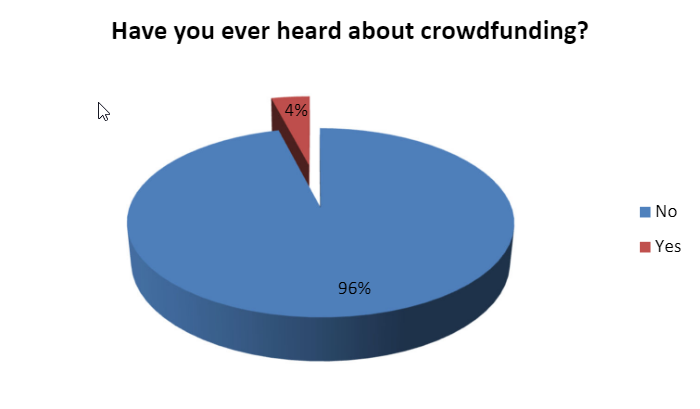
\includegraphics[scale=0.60]{assets/heardCrowd.png}
      \caption{ Have you heard of crowdfunding? }
      \label{fig:heardCrowd}
\end{figure}

\begin{figure}[!ht]
      \center
      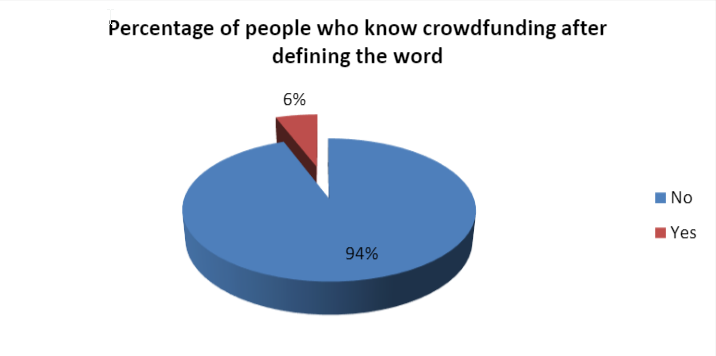
\includegraphics[scale=0.60]{assets/knowCrowd.png}
      \caption{After explaining the meaning of crowdfunding}
      \label{fig:knowCrowd}
\end{figure}

\begin{figure}[!ht]
      \center
      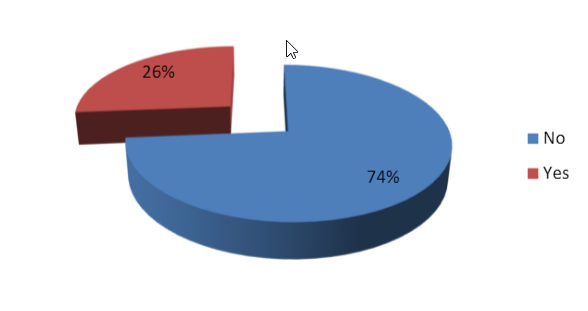
\includegraphics[scale=0.60]{assets/knowPlatform.png}
      \caption{Do you already know a crowdfunding platform?}
      \label{fig:knowPlatform}
\end{figure}

\begin{figure}[!ht]
      \center
      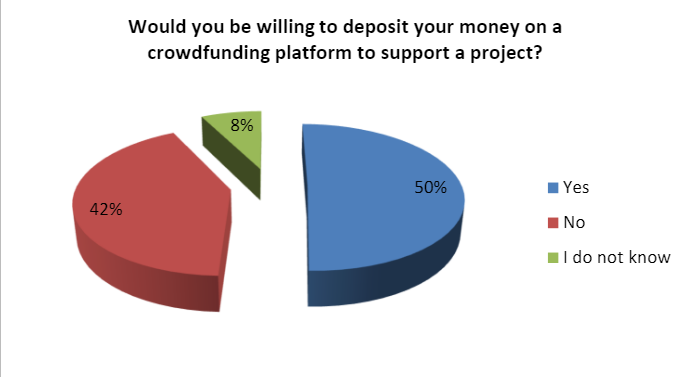
\includegraphics[scale=0.60]{assets/willing.png}
      \caption{Would you be to support a project on a crowdfunding platform?}
      \label{fig:willing}
\end{figure}



\section*{ Main Actors }
Different players are involved in crowdfunding models. First, many people propose ideas and
projects to be funded. They want to use crowdfunding as a tool to gather financial support from interested supporters.
Then there is the crowd of people that provides this financial support to these projects, bearing an investment
risk and expecting a certain payoff. And finally, there is the crowdfunding platform, the intermediary that acts
as a matchmaker between those who want to deliver the new initiatives using crowdfunding mechanisms
and those who want to support such initiatives through their investment efforts[\cite{10.1108/09564231111155079}]. In this chapter, we will
examine these three actors.

% In crowdfunding there is two main actors, the project owner that created the fundraiser, and the actor that provide the funds.
\begin{enumerate}
      \item Creator:
            Capital seekers are mainly concerned with their motivations to get involved in crowdfunding, the determinants of success, and the legal restrictions of equity-based crowdfunding[\cite{10.1007/978-3-319-18017-5_3}].

      \item Funder:
            Capital providers are essential to the success of a crowdfunding campaign. Interesting research can be performed on the motives of this unique group of investors for participating in crowdfunding. One thing that
            makes this group so special is that they are not exclusively motivated by earning money.

\end{enumerate}
\cleardoublepage%

% @Author: Taha Bouhsine


%%%%%%%%%%%%%%%%%%%%%%%%%%%%
% CHAPTER                  %
%%%%%%%%%%%%%%%%%%%%%%%%%%%%
\setcounter{mtc}{7}
\chapter{Project General Context }%
\label{chap:chapter_one}
\minitoc
%%%%%%%%%%%%%%%%%%%%%%%%%%%%
% SECTION                  %
%%%%%%%%%%%%%%%%%%%%%%%%%%%%
\section{ Project Presentation }
\subsection{Presentation}
Multiple projects and ideas all over the world go to waste and get canceled due to either lack or insufficient funds.
Which means the loss of a huge amount of new business chances and opportunities that would have been of great benefits for both individuals and communities.\\
The result is an extreme demand and concern to come up with a crowdfunding platform the necessary tools for the public to create, fund, and support causes and creative minds all over the world.



\subsection{Problem}
For the last few years, all over the world crowdfunding become one of the main tools and funding source for most of the new startups and creative minds all over the globe,
so we sought to create a new crowdfunding application, that will bring and adopt all the creative minds and ambitious souls and provides them with a tool to seek funds from a global community,
and help people to back and fund the creator in their journey and help him showcase the ideas that will be brought to life through the direct support of others.
so the creators will be able to coordinate multiple campaigns easier, and will be able to find people who are willing to invest with little equity involved.
And we sought also to provide a platform that will allow for gatekeeping that will monitor and create symbiotic relations with other algorithms and information online by using cloud-based solutions for better access.
our platform can help leap the hurdle of lack of experience in each field. Letting the barrier of entry be lessened for everyone who has a dream.\\

"Ideas are cheap, Execution is expensive" Even if you create a beautiful application with a beautiful User Interface, if you neglect even one aspect of the main functionalities, and built it with a half effort, you might result in a product that won't live for long, or if you were to use the wrong technologies for the project, you might as well find yourself limited and won't be able to create and bring the most out of your Idea.\\

So for our project, there is a real challenge in creating a product that competes with all the other platforms out there,
and first of all, we have to define what are the objectives we are seeking to complete to get to that final product,
so one main thing we needed to get our self doing is to look for the philosophies of crowdfunding, and try to understand humans motivation that make them want to fund and help another human, and what makes the creator seek funds from this type of fund seeking,
so we read some articles that have studied and handled the academic side of crowdfunding, from the university of  researchers create \cite{inproceedings}, which helped us in a great deal to understand the depth of our problem, and guided us into creating our application design, as some researchers whom are studying the psychology of giving seek to understand why certain people give and how to get more individuals to give.They suggest that goals, schema, information processing, memory, involvement, attitudes, affective processing, atmospherics, and consumer attributions and choices are the key elements of consumer behavior that drive the consumer decision process.
And that Creators are motivated to use crowdfunding platforms because it provides an easy, efficient, organized way to solicit and collect financial support from many people in a distributed network \cite{crowdMotiv}. By using web-based technologies, such as online payment systems and social media, creators are able to market and solicit resources safely and easily through crowdfunding platforms.

\subsection{Main Actors}
Different players are involved in crowdfunding models. First, there are creators, innovators, and entrepreneurs that have ideas and
projects to be funded. They want to use crowdfunding to gather financial support from interested supporters.
Then there is the crowd of people that provides this financial support to these projects, bearing an investment
risk and expecting a certain payoff. And finally, there is the crowdfunding platform, the intermediary that acts
as a matchmaker between those who want to deliver the new initiatives using crowdfunding mechanisms
and those who want to support such initiatives through their investment efforts \cite{crwdfun:transform}.
% Creators
\subsubsection*{Creators}
The reasons for people to fund their projects via crowdfunding are wider than just money. Gerber et al. \cite{inproceedings} 
have, by interviewing people involved in crowdfunding, identified the following motivations:
\begin{enumerate}
      \item Raise Funds: 
            Almost trivial, one of the motivations is to raise funds. Also, platforms provide a way to
            collect payments online, and accept small payments from a large number of people. Therefore, capital
            seekers do not need to develop an infrastructure for it.

      \item Establish Relationships and form Connections:        
            In addition to raising funds, one other advantage is the opportunity for a direct
            connection between creators and funders potentially extending beyond the campaign itself. The
            long term relationship stands in contrast to the short term relationship that occurs in many alternatives
            to crowdfunding.

      \item Maintain Control.

      \item Learn New Fundraising Skills.

      \item Receive Validation and approval:           
      Successful experiences and receiving public recognition of their success increase
            a person’s confidence in his/herself and the project. According to the writers, this finding is consistent
            with social cognitive theory, which suggests that people build beliefs in their ability through social interactions. This finding is supported by prior research in online communities, which finds that people
            engage in these communities to build self-esteem.

      \item Replicate Successful Experience of Others:          
            According to the researchers, initial findings suggest that
            people participate in crowdfunding because they want to replicate the success of others. Creators that
            succeed in funding a project online provide social proof that motivates others to become creators as
            well.

      \item Expands Awareness  of Work  through Social Media:     
            Findings suggest that creators were motivated to
            participate in crowdfunding because it expanded their awareness through social media. In one of the
            interviews in the research, an anthropologist who used the crowdfunding platform RocketHub to fund
            her research on ancient Roman skeletons, described being motivated to not only share her work publicly but engage in a dialogue about her work. She gained a lot of followers on Twitter and has even
            started a blog as a result of her newfound fame.

\end{enumerate}

Creators deterrents to Crowdfunding:
\begin{enumerate}
      \item Inability to Attract Supporters
      \item Fear of Public Failure and Exposure
      \item Time and Resource Commitment
\end{enumerate}

\paragraph*{Factors For Successful Crowdfunding}
\begin{enumerate}
      \item Orientation of the project:     
      Whether the project or the organization behind it is a non-profit or not
            seems to influence the success of funding. Belleflamme et al. \cite{doi:10.1080/13691066.2013.785151} performed an empirical analysis
            to investigate this. They found that non-profit organizations tend to attract larger amounts of money.
            According to them, this finding is in line with earlier research stating that non-profit organizations
            are better at attracting outside funds because of their stronger focus on the social outcome than on
            monetary gains.

      \item Amount and duration:     
      According to that same research \cite{doi:10.1080/13691066.2013.785151}, increasing goal size is negatively associated
            with success. Less expected was that an increased duration of a campaign decreases the chances of
            success. This might be explained as that longer durations are a sign of lack of confidence.

      \item Social network:     
      Research by Agrawal et al. \cite{NBERw16820} indicates the important role that friends and family may
            play in generating early investment in entrepreneurial ventures. They speculate that this early investment may serve as a signal of entrepreneurial commitment. Later investors may use this signal thereby
            increasing the likelihood of further funding by way of access to distant sources of capital.
\end{enumerate}


% Funders
\subsubsection*{Funders}
Funders are essential to the success of a crowdfunding campaign. Interesting research can be performed on the motives of this unique group of investors for participating in crowdfunding. One thing that
makes this group so special is that they are not exclusively motivated by earning money.
In crowdfunding, consumers have taken on the role of investors or capital providers. And they are diverse. Even on the same platform, the motives to make investments can greatly vary between consumers.
Based on earlier research, Lin et al. \cite{doi:10.5465/ambpp.2014.209} have identified a set of motivations that may drive a person’s participation in crowdfunding:

\begin{enumerate}
      \item Seek Rewards:
            At reward-based platforms such as Kickstarter or Indiegogo, capital seekers can offer rewards linked to the size of the contribution by the investor. These rewards range from t-shirts and
            acknowledgment on the project page to pre-ordering the actual product. The latter sometimes leads
            to confusion situations for consumers. Although explicitly disclaimed by Kickstarter, many consumers
            are under the impression that the web site is essentially an online retail storefront in which project
            creators are pre-selling products \cite{10.2139/ssrn.2234765}.

      \item Help Others and support Creators and causes: One of the interviewees from a study carried out by Gerner et al. \cite{inproceedings}
            stated that he funds an idea that he thinks is neat, but he also really likes the idea of people being
            able to get off the ground without needing to buy into a big giant corporate structure.

      \item Engage and Contribute to a Trusting and Creative Community:
            A crowdfunding platform’s senior executive noted that the way the crowdfunding model works is that people generally feel like they are involved or engaged in the project
            throughout the duration. Crowdfunding allows a lot of people to be involved in something that
            they maybe otherwise would not have the opportunity to be involved in. Just to be a part of something
            is what motivates people in those cases \cite{inproceedings}.

      \item Reputation:
            Another motivation for many participants of online and crowdsourcing communities is
            the reputation benefits and recognition that can be derived from active participation in the community \cite{doi:10.5465/ambpp.2014.209}.
            Fellow investors on Kickstarter can see what projects you backed. This creates a sense of ’high-profile
            community members’.
\end{enumerate}


One motivation of supporters in crowdfund-ing communities is the desire to collect external rewards such as an acknowledgment, a tangible artifact, or an experience. An acknowledgment may come in the form of a telephone call, while a tangible artifact could be a CD or gadget. An experience may involve, for instance, meeting with the creator. The creator’s goal is to provide rewards that satisfy the supporters’ desire to collect.

\subsection{Design Principles}
Based on these motivations, Gerber et al. \cite{crowdMotiv} developed three design principles for crowdfunding
intermediaries. These principles enhance motivation for these actors to individually decide to become and
stay involved in crowdfunding.

\subsubsection*{Support Resource Export}
Crowdfunding actors should be able to exchange human, information, and financial resources before, during, and after the crowdfunding campaign. The human resources are persons that can help to fulfill tasks
associated with creative production, such as creation, manufacturing, implementation, marketing, planning,
and fulfilling. Often creators do not have experience in all these fields. Therefore it can be useful to find
an advisor or even a companion. Examples of information resources are information and explanations. Access to informational and human resources has been found to have a direct positive impact on persistence
in ambiguous tasks. With financial resources, we refer to funding. Almost all platforms already provide the
exchange of financial resources, as this is fundamental to crowdfunding. The exchange of the other types are
often overlooked. Adding this to the design could potentially enhance a project’s success.
During the preparation stage, capital seekers are advised to search for example projects, read advice blogs,
seek one-on-one advice, and outsource preparation tasks. However, on many intermediaries, users cannot
see unsuccessful campaigns \cite{10.1145/2531602.2531715}.

\subsubsection*{Support community before, during, and after}
Intermediaries could offer users the possibility to interact or meet up before, during, and after the campaign.
There should be opportunities to meet up with potential capital providers to increase awareness of the upcoming project before the campaign starts. During the campaign, there should be tools and channels available to promote the project. And when the campaign is successful, there should be a way to keep supporters
up-to-date about the execution of the project. Because current platforms do not all sufficiently support this,
users often go to external communities such as Reddit.
According to earlier research, people are more likely to persist when they publically commit beforehand
and then share small wins with others throughout the effort. Through the sharing process, they receive positive validation and are more likely to believe they can accomplish a task, are willing to take on more challenging work, have a greater intrinsic motivation to complete a task, persist in the face of challenges, and expend
more effort in the task \cite{crowdMotiv}.
The community around crowdfunding developed tools to support after-campaign work. One example
is Backerkit, which allows project creators to organize supporter and reward information. Another example
called Fullfillrite manages crowdfunding reward shipping efforts. Intermediaries could offer a matchmaking
service to bring together supply and demand \cite{doi:10.5465/ambpp.2014.209}.
% \subsubsection*{Provide transparency}
% On crowdfunding intermediaries, capital seekers pitch their unique ideas to the crowd. The legalities involved
% should be included in the sign-up process. It is important that this is done in a way that is understandable for
% non-experts. Providing a 20-page-long document with all the rules in a language only lawyers can understand
% is not suggested. The same goes for the legalities involved when intermediaries are collecting data on their
% users. Research in psychology and human-computer interaction suggests that transparency creates trust,
% and trust supports future participation.

\subsection{Objectives}

So one of our main objectives is to create a platform that can improve our user's experience and boost the chance of our creators to reach the maximum of the audience as well as facilitate the access and the funding process for our funders, and provide a place where they can build there trust and look for promising talents and empowering entrepreneurs to help in creating new possibilities.\\

Firstly, we need to make sure
that the code is maintainable for future alterations and additions by other programmers. For this, we will try
to keep the files organized in a logical setup and we will comment our code where necessary, to understand
its workings.\\

Secondly, Sahem platform will deal with sensitive data on several occasions. First of all, there
is the user data, which includes personal information and passwords. Secondly, there is a payment system
that involves sensitive financial information of the users. This is why it is very important to build our system
to be as secure as possible.\\

Thirdly, the platform needs to have an attractive and clean design. It needs to be user-friendly, easily navigable, and look professional so that users will trust the platform is capable of performing
well in the financial setting. So I came up with a unique design, and tried to create a new experience for the users, fast,
smooth, mobile responsive, and easy interface to interact with.
\begin{enumerate}
      \item
            User Experience:
            Making sure that our crowdfunding software solutions are easy to navigate for the end-user is a crucial part of the development process. If our customers are befuddled by how to navigate our application, then it is highly likely that they will leave and find another crowdfunding platform. Not only will we want a functional interface, but one that is eye-catching as well.
            One thing to take note of is the importance of giving them the terms and conditions within the first few steps, so they fully understand what to expect. This shows a dedication to transparency that many startups and entrepreneurs will appreciate.

      \item
            Account Management:
            Our customers will want to know what is going on, and making it easy on them will help make our platform successful. That means setting up systems that make it very clear what’s going on with their project. We will want them to be able to access who has been investing, how much money they have, how far they are from their goal, and any other metric they need to run a successful campaign. This could also include reports for recharges, withdrawals all available via a simple to navigate dashboard.
      \item
            Report Generation:
            As the platform owner, you need a way to benefit from your time spent on creating this site that will help so many people. So, ensuring you also have access to backed reports like rewards, investors, and such can help you help them, as they say. This means creating a dashboard that, just like for the actual campaign creators, is easy to navigate and gives you access to reports you can use to course-correct and upgrade the systems.
      \item
            Payment Gateway \& Marketing:
            When starting a crowdfunding platform you will want to set it up with access to the right payment gateways. Each gateway has its features, and so doing some in-depth research into them will allow you to choose one or several that works for the largest number of potential customers.
\end{enumerate}



\section{Functionality}
The platforms operate by allowing those seeking finance to make a pitch on the site outlining how much money they need, what they need the money for, if anything, you get in return for contributing. Potential funders can then view pitches on the platform, interact with both those looking for finance and other potential funders, and then decide whether or not they want to back the campaign. The majority of platforms operate the all–or–nothing model where, if the target amount is not raised within a given timeframe, contributions are returned to funders and no financing goes ahead, but we are using the Keep It All model, anything you raise is yours.\\

When a new user arrives at the landing page he will be greeted with the main interface of the application, that holds multiple pieces of information and presentations of our platform, it explains the basic functionalities and the different advantages of our application.\\

Our simple design, based on some principles of improving the user's experience found in Krug's book "Don't make me think, revisited: a common sense approach to Web usability", we have chosen to make the most important buttons into unique color from the others, on normal cases the user will click on one of them to navigate to the appropriate page, at first he will have the ability to navigate to the existing fundraiser campaigns of the platform, and if he chooses to fund the project, he will be redirected to the Registration form in order to authenticate, and fill his personal profile, and provide the platform with his credit card information.\\

After the authentication, he will have the ability to create and submit his own fundraiser.\\

In his profile, he can see his personal information and get to show all of his achievements, the projects he funded, and the fundraisers he created as well as the posts he published in the platform. 
% TODO 

\section{Feasibility}
This project is technically and financially feasible. I will spend approximately nothing to host the app, and in the future, there is an option to pay as you grow, by generating income from cutting a \% from the funds at the end of each fundraiser, we will get the costs covered. With regards to the technical feasibility, it will be built in well-established MEAN Stack technologies, that have a low cost with great scalability, and maintainability.

Sahem provides the following features:
\begin{enumerate}
      \item Trust-building through the corroboration mechanism.
      \item
            Opportunity for long term commitment between Creators and Funders.
      \item
            Uses secure technologies on both the frontend and the backend, and any requests sent by the users are passed by multiple middlewares on the backend.
      \item
            Easy Navigation through simple user interface design built using Angular, a framework that helps in creating fast and reliable Single Page Applications.
      \item
            A headless backend, which allow us to create different frontend application afterward, and that are linked to the same backend.
      \item
            Global crowdfunding interaction, no limits between countries, everyone can fund or create fundraisers.
      % \item
      %       Statistical analysis of need vis-à-vis people.
\end{enumerate}
\section{ Project Management }
Process-driven software development is based on rigorously defined activities and tasks that are also repeatable and measurable. Formal processes facilitate planning, analysis of requirements from multiple angles, design of high-quality software models by following standards and using team-based tools, and incorporation of quality through walkthroughs, inspections, and testing.

As a result, such formal processes enhance quality and maximize user benefits.
\subsection{ Project Development Process }
The process of discipline is complex. This is because a process considers myriad different hard and soft factors that impact development. Many software developers argue that processes restrict their creativity. Far from that, processes enable creativity with value. This is because processes ensure the effort made by architects, designers, developers, and testers will be well directed toward the commonly agreed goals (business objectives) of a project. Processes also facilitate measures and metrics that indicate individual and team productivity and quality. Metrics and measurements in software projects also enable the assignment of responsibilities and accountabilities.
To develop a good product we need a good development method. One very popular agile framework for this is iterations and increments.\\

The iterations and increments as shown in Figure \ref{fig:iterationlifecycle} are the basis of most modern-day approaches to developing good software. In this iterative and incremental approach, no deliverable is produced in a single attempt. Instead, at least three iterations (repetitions) are undertaken before producing a deliverable.
This is followed by incrementally adding another package, which would have its own three or more iterations. The three terms iteration, incremental, and parallel are further discussed next.
\begin{figure}[!ht]
      \center
      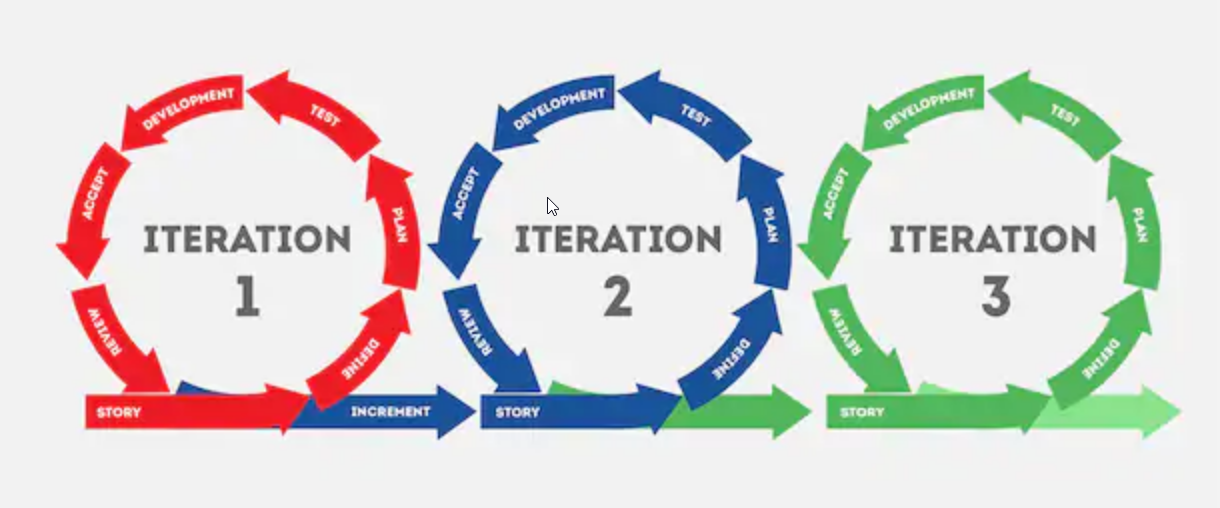
\includegraphics[scale=0.40]{assets/iteration.png}
      \caption{Iterative process project life cycle}
      \label{fig:iterationlifecycle}
\end{figure}
\paragraph*{Iterative}
The iterative aspect of a process enables the repetition of tasks. As a result, the deliverables are produced gradually. For example, when a use case is iterated, additional material is added to the description of the use case—such as alternative flows within the use case. The iterative approach encourages a slow and steady philosophy rather than hurrying and finishing up a deliverable in the first attempt.
Deliverables are gradually matured by undertaking at least three iterations across multiple other deliverables. For example, while following an iterative process one might move from an initial use case to another use case in another diagram, then identify classes and draw a sequence diagram before coming back to the original use case and completing it.
\paragraph*{Incremental}
The incremental aspect of a process enables adding new elements and diagrams to an existing deliverable. An example is to add new packages to existing or developing packages. New requirements are thus discovered and modeled incrementally. This incremental aspect of the process enables the creation of parts of a system in as complete a manner as possible before proceeding with the development of additional parts of the system. The incremental aspect of a process often goes hand in hand with the iterative aspect. For example, while a new deliverable is incrementally added (a new use case), an existing deliverable is iteratively augmented during a later iteration (e.g., additional steps added to a use case).
\clearpage
\subsection{Monitoring And Planning}
\subsubsection*{Monitoring}
Breaking down a project into subparts does help a lot in enabling controlled the execution and monitoring of the project, it helps with keeping the project well displayed and well planned to avoid all the mishaps spaghetti code afterward.\\
Figure \ref{fig:bos} shows how we divided the business objective into subparts. To arrive at acceptable performance criteria of the system, the BO gets further divided into smaller parts or subject areas.
\begin{figure}[!ht]
      \center
      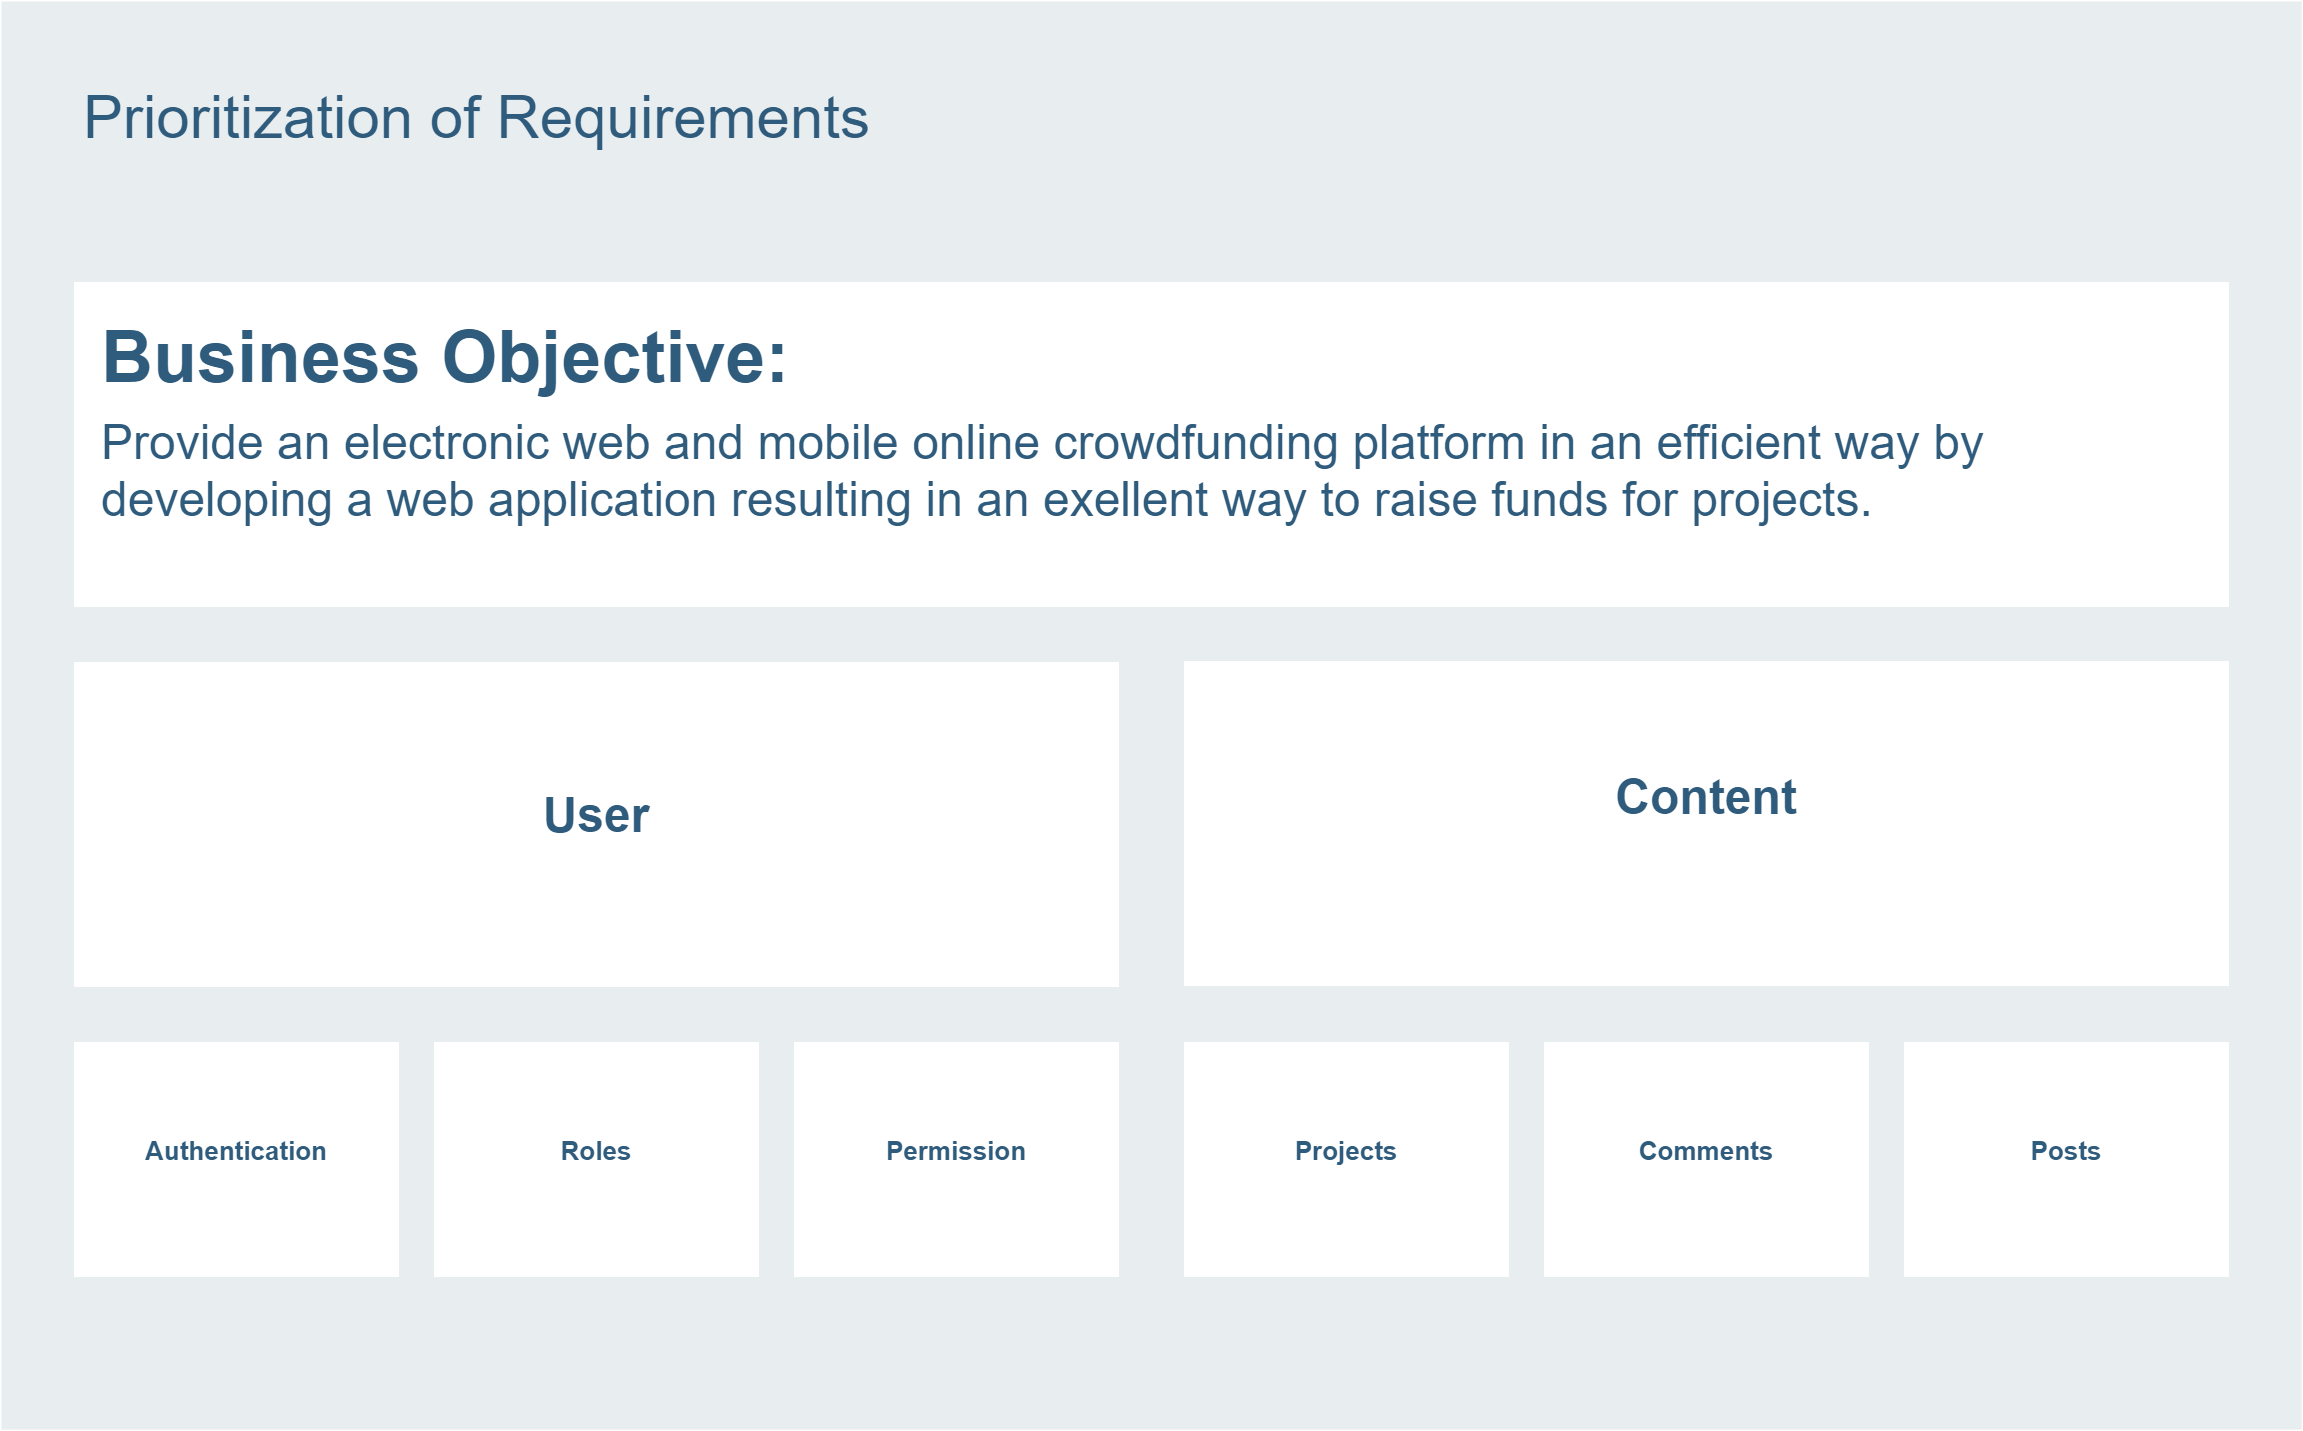
\includegraphics[scale=0.18]{assets/bos.png}
      \caption{Sahem's Business Objectives}
      \label{fig:bos}
\end{figure}
\subsubsection*{Planning}
During the planning we should provide precise routing of one or more business processes with opportunities to optimize on time and costs associated with the processes.
So we created a Gantt Chart in teamGantt to help us follow the progress of different tasks and the time left to complete them:
% what we did with gantt chart
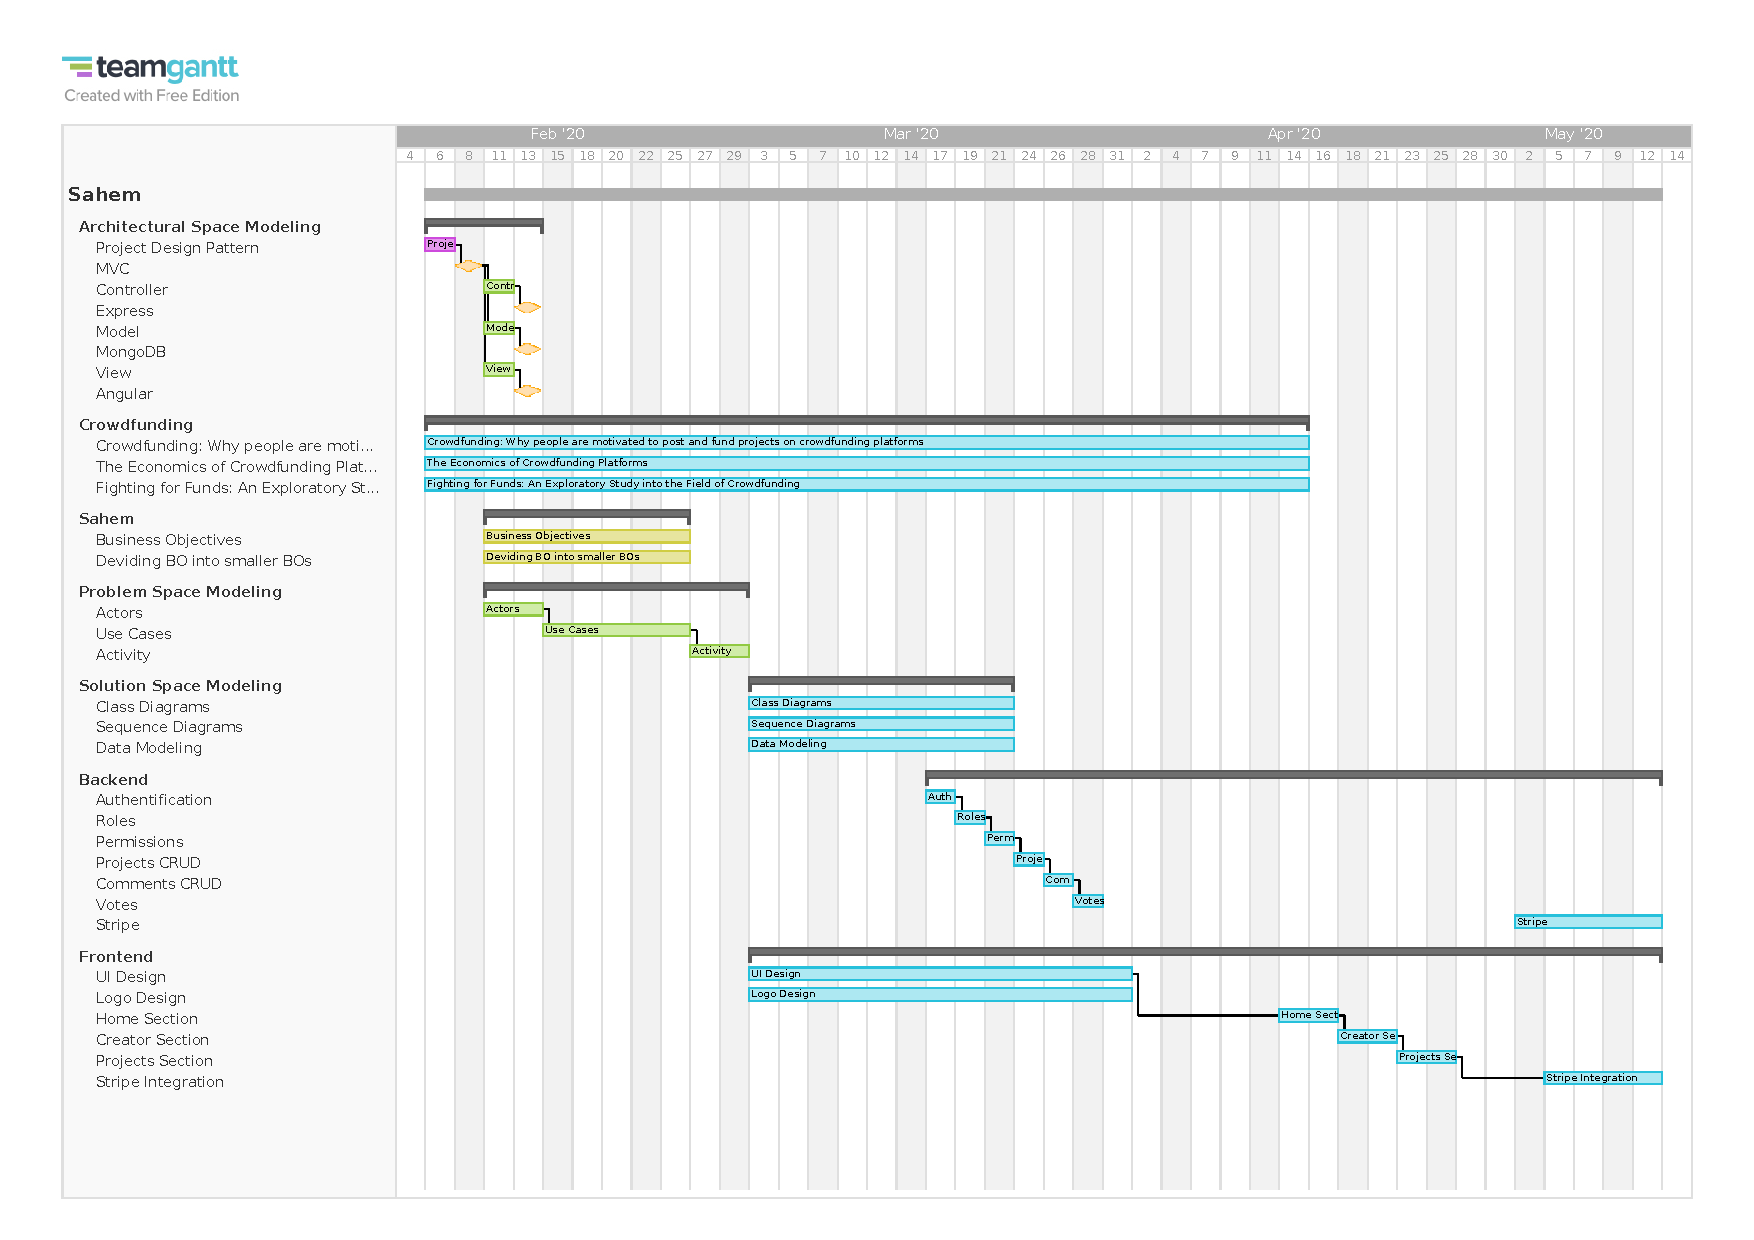
\includepdf[pages=-,angle=90,]{assets/ganttchart.pdf}

\cleardoublepage%

% @Author: Taha Bouhsine


%%%%%%%%%%%%%%%%%%%%%%%%%%%%
% CHAPTER                  %
%%%%%%%%%%%%%%%%%%%%%%%%%%%%
\setcounter{mtc}{8}
\chapter{Analysis And Design}%
\label{chap:chapter_two}
\minitoc
%%%%%%%%%%%%%%%%%%%%%%%%%%%%
% SECTION                  %
%%%%%%%%%%%%%%%%%%%%%%%%%%%%
\section{General description of the platform}

% \begin{description}\addtolength{\itemsep}{-0.35\baselineskip}%
%   \item[\textbullet~\bfseries Menu Item] \hfill \\%
%         Menu Description.~\\%
%         {\textbf{Focus topics:~}\emph{Topic one, topic two, topic three, ...}}%
%         %
%   \item[\textbullet~\bfseries Menu Item] \hfill \\%
%         Menu Description.~\\%
%         {\textbf{Focus topics:~}\emph{Topic one, topic two, topic three, ...}}%
%         %
%   \item[\textbullet~\bfseries Menu Item] \hfill \\%
%         Menu Description.~\\%
%         {\textbf{Focus topics:~}\emph{Topic one, topic two, topic three, ...}}%
% \end{description}

% Also bullets such as:%
% \begin{itemize}\addtolength{\itemsep}{-0.35\baselineskip}%
%   \item One%
%   \item Two%
%   \item Three%
%   \item Four%
%   \item \ldots%
% \end{itemize}%
% %

\section{Specification of requirements}
We will proceed according to the UML method which consists of identifying and modeling the various business processes in order to easily migrate to an object architecture from a static and dynamic point of view. This analysis presents a total abstraction being independent of any technology or implementation.

The specification of the needs will allow us to have a better approach of the users, the functionalities, and the relationship between the two. It will be in the form of a use case. For this we will proceed as follows:

Identification of requirements.
Identification of the actors of the system.
Identification of use cases.
Description of use cases.
Grouping of use cases into packages.


\subsection{requirements}
The requirements that we have put on the end-product were divided into basic functionalities and optional functionalities.
The User’s basic functionalities are:
\begin{enumerate}
    \item
          Account management: create an account, login, profile, settings, personal info,
          personal dashboard.
    \item
          Start a campaign: send in a proposal for a campaign (webform).
    \item
          Share function: functionality so that a campaign can be shared within social networks, such as Facebook, Instagram, LinkedIn, Twitter, and potentially Pinterest and Google.
    \item
          Contribution invitation: functionality to send out concrete requests to contribute a certain amount
          within the personal social network.
    \item
          Payment function: contributor should be able to pay their ticket through Credit Card.
    \item
          Review function: contributors should have the opportunity to give reviews about and react to events
          that have taken place.
    \item
          Countdown timer: a timer that shows how much time a campaign has left until it closes.
    \item
          Current overview: each campaign should show for example the number of tickets sold/amount of investors, the amount of money raised so far and the goal amount to be raised.
\end{enumerate}


The User’s optional functionalities are:

\begin{enumerate}
    \item
          Personalized recommendations (recommender system): the system will advise, suggest, or give concrete offers. Logged-in visitors see a personalized recommendation based on social profiles and the
          platform’s web page content and actions.
    \item
          Share option via Whatsapp
    \item
          Online helpdesk: chat possibility with a helpdesk worker.
    \item
          Communication tools: communication possibilities with other members and/or the organization of an
          event via chat.
    \item
          Connection with social media: e.g. Facebook application for special opportunities and/or campaigns
          that enabled even more interaction with the target group.
    \item
          Social login: login with a social account.
    \item
          Wallet: deposit money in your personal wallet, which enables you to make several contributions by
          paying with the money in your wallet.
    \item
          Recruit function: a tool to gather more contributors. A contributor can share a campaign within their
          own personal social networks.
    \item
          Notifications: reminders and/or messages related to upcoming events and updates of events.
    \item
          Mobile App: extra functionalities through the use of a camera and GPS on the actual event: e.g. picture/video upload to the website or live visitor numbers.

    \item
          Agenda/calender: an overview that shows which events will take place on which dates (including events
          that have already taken place).
    \item
          Newsletter: send an overview of the events to members of the platform community or a certain
          selection.
    \item
          Promotion function: functionality to share and promote events on different levels: community (everyone), events (only participants of a specific event), social media (within social networks).
    \item
          Campaign management: management tools for the event organization.
    \item
          Reports/statistics: data analyses, tools for advanced analysis of the web page visits.
\end{enumerate}




\subsection{Identification of actors}
In UML we don't use the term users but actors. A player in a system is an entity external to this system that interacts (data entry, reception of information, etc.) with it. The actors make it possible to define the interface that the system will offer to its environment. And also the actor groups together several users who have the same role. And to find actors it will be necessary to identify the different roles that will have to play its users.
In order to facilitate identification, we can imagine this: everything that is outside and interacts with the system is an actor, everything that is inside is a functionality to be realized.
The different actors of the studied system are \ref{fig:sahemactors}:
\begin{figure}[!ht]
      \centering
      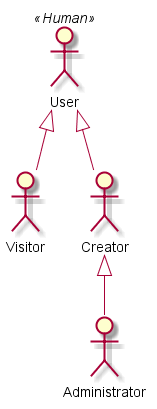
\includegraphics[scale=0.60]{assets/Actors.png}
      \caption{Sahem Platform Actors}
      \label{fig:sahemactors}
\end{figure}
\begin{enumerate}
    \item  Creator.
    \item  Funder will be merged with Creators.
    \item  Administrator.
    \item  Visitor.
\end{enumerate}

\subsection{Identification of objectives and use cases}
A use case described in the form of actions and reactions, the behavior of a system from a user point of view. It must add value to the actor concerned. Each use case contains a list of functionalities that will be detailed in the following section.

We will first determine the objectives that will allow us to deduce the use cases and all this:
\begin{longtable}{|m{10em}|m{10em}|m{10em}|}\hline
    \multirow{4}{*}{Administration management} & \multirow{2}{*}{Authentication}       & Authentication                          \\\cline{3-3}
                                               &                                       & Registration                            \\\cline{2-3}
                                               & \multirow{5}{*}{User Maintainance}    & Add User                                \\\cline{3-3}
                                               &                                       & Modify User                             \\\cline{3-3}
                                               &                                       & Delete User                             \\\cline{3-3}
                                               &                                       & Consult the information of a user       \\\cline{3-3}
                                               &                                       & Show the list of users                  \\\cline{2-3}
                                               & \multirow{2}{*}{Roles}                & Show users by roles                     \\\cline{3-3}
                                               &                                       & Modify a user's role                    \\\cline{2-3}
                                               & \multirow{1}{*}{Statistics}           & Access the statistics of the plateforme \\\hline
    \multirow{4}{*}{Fundraiser's managment}    & \multirow{3}{*}{Creator's Monitoring} & Personal information modification       \\\cline{3-3}
                                               &                                       & Access a creator profile                \\\cline{3-3}
                                               &                                       & Desactivate an Account                  \\\cline{2-3}
                                               & \multirow{2}{*}{Funds Monitoring}     & Fund a project                          \\\cline{3-3}
                                               &                                       & Confirm funding a project               \\\cline{3-3}
                                               &                                       & List of previous funds                  \\\cline{2-3}
                                               & \multirow{6}{*}{Projects Monitoring}  & Create a project                        \\\cline{3-3}
                                               &                                       & Edit a project                          \\\cline{3-3}
                                               &                                       & Delete a project                        \\\cline{3-3}
                                               &                                       & Like a project                          \\\cline{3-3}
                                               &                                       & Share a project                         \\\cline{3-3}
                                               &                                       & Comment on a project                    \\\cline{2-3}
                                               & \multirow{2}{*}{Search}               & Search a project by name                \\\cline{3-3}
                                               &                                       & Show Fundraisers by category            \\\hline
    \multirow{2}{*}{Payment management}        & \multirow{1}{*}{Billing}              & Show the bill                           \\\cline{2-3}
                                               & \multirow{1}{*}{Online Payment}       & Choose payment method                   \\\hline

    \caption{Identification of objectives and use cases}
    \label{tab:id_objec_uc}
\end{longtable}

%%%%%%%%%%%%%%%%%%%%%%%%%%%%
% SECTION                  %
%%%%%%%%%%%%%%%%%%%%%%%%%%%%
\section{Analyse fonctionnelle}
usecase
%%%%%%%%%%%%%%%%%%%%%%%%%%%%
% SECTION                  %
%%%%%%%%%%%%%%%%%%%%%%%%%%%%
\section{Analyse dynamique}
activity  squence
%%%%%%%%%%%%%%%%%%%%%%%%%%%%
% SECTION                  %
%%%%%%%%%%%%%%%%%%%%%%%%%%%%
\section{Analyse structurelle}
class
\cleardoublepage%

% @Author: Taha Bouhsine


%%%%%%%%%%%%%%%%%%%%%%%%%%%%
% CHAPTER                  %
%%%%%%%%%%%%%%%%%%%%%%%%%%%%
\setcounter{mtc}{9}

\chapter{Technical and environmental study}%
\label{chap:chapter_tree}
\minitoc
\section{Capture of technical needs}
The capture of technical needs identifies all the constraints and the choices dimensioning the design of the system.

The tools and materials selected as well as the management of integration constraints generally conditioning the prerequisites of general architecture.

The capture of technical needs is as follows:
\begin{itemize}\addtolength{\itemsep}{-0.35\baselineskip}
      \item
            Capturing software specifications.

      \item
            Capturing specifications related to hardware configuration.

\end{itemize}

\subsection{Capturing software specifications}
Once the hardware specifications have been determined, we move on to the non-functional specifications, in other words, technical or software specifications.

These are technical features that the system will provide to the user regardless of the business or functional term.

We will, therefore, list a list of technical functionalities that our system will be able to provide and offer to users, which is why we have introduced the concepts of operator and technical use cases:

\paragraph{Technical actors}
Also called "technical actors" of the system, these are the actors who benefit from the technical functionalities of the system:
\begin{itemize}\addtolength{\itemsep}{-0.35\baselineskip}
      \item
            User: These are the people who use the system functionality in one way or another.
      \item
            Administrator: this is the person responsible for managing all the management of the platform as well as that of the users.
\end{itemize}

\paragraph{Identification of technical use cases}

\begin{longtable}{|m{10em}|m{10em}|m{10em}|}\hline
      \multirow{4}{*}{Security management} & \multirow{5}{*}{Authentication}          & UC1-Register                                                    \\\cline{3-3}
                                           &                                          & UC2-Login                                                       \\\cline{3-3}
                                           &                                          & UC3-Reset Password                                              \\\cline{3-3}
                                           &                                          & UC4-Change password                                             \\\cline{3-3}
                                           &                                          & UC5-Logout                                                      \\\cline{2-3}
                                           & \multirow{1}{*}{Confidentiality}         & UC6-Role management                                             \\\cline{2-3}
                                           & \multirow{2}{*}{Secure payment}          & UC7-Send Payment                                                \\\cline{3-3}
                                           &                                          & UC8-Receive Payment                                             \\\cline{2-3}
                                           & \multirow{2}{*}{Backup and restore}      & UC9-Save the database                                           \\\cline{3-3}
                                           &                                          & UC10-Restore the database                                       \\\hline
      \multirow{7}{*}{Data managment}      & \multirow{1}{*}{Dynamic data}            & UC11-Dynamic data dispaly                                       \\\cline{2-3}
                                           & \multirow{1}{*}{Integrity}               & UC12-Simultaneous updates                                       \\\cline{2-3}
                                           & \multirow{1}{*}{Interoperability}        & UC13-Network deployment                                         \\\cline{2-3}
                                           & \multirow{1}{*}{Compatibility}           & UC14-Run on different browsers and platforms                    \\\cline{2-3}
                                           & \multirow{2}{*}{History}                 & UC15-Get all the user created projects fundraised               \\\cline{3-3}
                                           &                                          & UC16-Get all the user created projects fundraised               \\\cline{2-3}
                                           & \multirow{1}{*}{Statistics}              & UC17-Display platform statistics                                \\\cline{2-3}
                                           & \multirow{1}{*}{Fund}                    & UC18-Fund migration from anonymous user                         \\\hline
      \multirow{4}{*}{Help management}     & \multirow{2}{*}{Gestion des erreurs}     & UC19-Logging Viewing types of errors                            \\\cline{3-3}
                                           &                                          & UC20-Send the error by email to the administrator               \\\cline{2-3}
                                           & \multirow{1}{*}{Aide en ligne}           & UC21-Consult the user help Guide                                \\\cline{2-3}
                                           & \multirow{1}{*}{Notifications}           & UC22-Confirmation or error message                              \\\cline{2-3}
                                           & \multirow{1}{*}{Mails}                   & UC23-Sending emails                                             \\\hline
      \multirow{2}{*}{Payment management}  & \multirow{1}{*}{Multi-currency platform} & UC24-Choose a currency for purchase and payment                 \\\cline{2-3}
                                           & \multirow{1}{*}{Payment method}          & UC25-Possibility to choose a payment method                     \\\hline
      \multirow{3}{*}{Optimization}        & \multirow{1}{*}{Navigation}              & UC26-Nested operations                                          \\\cline{2-3}
                                           & \multirow{1}{*}{Sharing}                 & UC27-Possibility to share your donation                         \\\cline{2-3}
                                           & \multirow{1}{*}{Theming}                 & UC28-Possibility to switch themes between dark and light themes \\\hline

      \caption{Identification of technical objectives and use cases}
      \label{tab:id_tech_objec_uc}
\end{longtable}

\paragraph{ Technical description use cases }
View all the use cases described in the appendix \ref{sec:ucd}


\subsection{Capturing hardware specifications}

\begin{figure}[!ht]
      \centering
      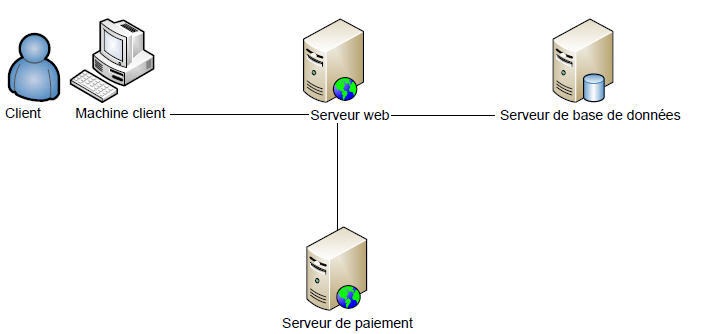
\includegraphics[scale=0.60]{assets/network-arch.jpg}
      \caption{Sahem Platform Actors}
      \label{fig:sahemactors}
\end{figure}

\section{Adopted Architecture}

\subsection{Model View Controller Design Pattern}

The Model View Controller (MVC) design pattern specifies that an application consists of a data model, presentation information, and control information. The pattern requires that each of these be separated into different objects.

MVC is more of an architectural pattern, but not for a complete application. MVC mostly relates to the UI / interaction layer of an application. We’re still going to need a business logic layer, maybe some service layer and data access layer.
\begin{enumerate}
      \item Model contains only the pure application data, it contains no logic describing how to present the data to a user.
      \item View presents the model’s data to the user. The view knows how to access the model’s data, but it does not know what this data means or what the user can do to manipulate it.
      \item Controller exists between the view and the model. It listens to events triggered by the view (or another external source) and executes the appropriate reaction to these events. In most cases, the reaction is to call a method on the model. Since the view and the model are connected through a notification mechanism, the result of this action is then automatically reflected in the view.
\end{enumerate}

\begin{figure}[!ht]
      \center
      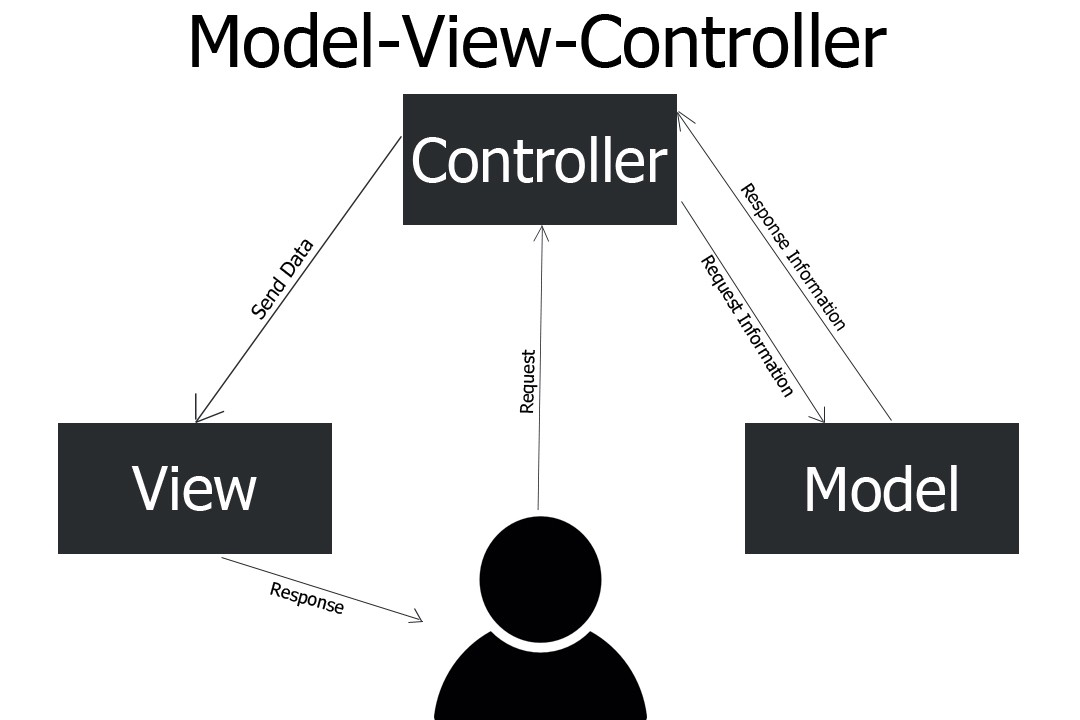
\includegraphics[scale=0.30]{assets/mvc.jpg}
      \caption{Model View Controller}
      \label{fig:mvc}
\end{figure}
% %%%%%%%
\subsection{Representational State Transfer Architecture}
REST, or REpresentational State Transfer, is an architectural style for providing standards between computer systems on the web, making it easier for systems to communicate with each other. REST-compliant systems, often called RESTful systems, are characterized by how they are stateless and separate the concerns of client and server. We will go into what these terms mean and why they are beneficial characteristics for services on the Web.
%%%%
\subsection{Software as a Service}
Software as a Service or SaaS , which allows us to set up services, such as application servers and databases, as needed to create the apps we need. This type of system typically works in a cloud or hybrid cloud environment, which often makes provisioning of servers and software as simple as entering some configurations and clicking a button.

This type of setup is perfect for the MEAN stack, as each piece of the MEAN stack is easily placed into the cloud and thus can be easily provisioned, so they are widely available on SaaS services and can be used quickly when needed. If we are looking for a good development stack, the MEAN stack has much to offer for IT management as well as for developers!
%%%%

\subsection{Monolithic Applications}

If all the functionalities of a project exist in a single codebase, then that application is known as a monolithic application. We all must have designed a monolithic application in our lives in which we were given a problem statement and were asked to design a system with various functionalities. We design our application in various layers like presentation, service, and persistence and then deploy that codebase as a single jar/war file. This is nothing but a monolithic application where “mono” represents the single codebase containing all the required functionalities.
\begin{figure}[!ht]
      \center
      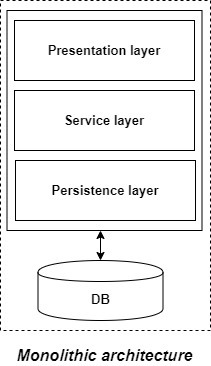
\includegraphics[scale=0.60]{assets/monolithic.jpg}
      \caption{Monolithic Applications}
      \label{fig:monoapp}
\end{figure}

Disadvantages of Monolithic applications:
\begin{enumerate}
      \item
            It becomes too large with time and hence, difficult to manage.
      \item
            We need to redeploy the whole application even for a small change.
      \item
            As the size of the application increases, its start-up and deployment time also increases.
      \item
            For any new developer joining the project, it is very difficult to understand the logic of a large Monolithic application even if his responsibility is related to a single functionality.
      \item
            Even if a single part of the application is facing a large load/traffic, we need to deploy the instances of the whole application in multiple servers. It is very inefficient and takes up more resources unnecessarily. Hence, horizontal scaling is not feasible in monolithic applications.
      \item
            It is very difficult to adopt any new technology which is well suited for a particular functionality as it affects the whole application, both in terms of time and cost.
      \item
            It is not very reliable as a single bug in any module can bring down the whole monolithic application.
\end{enumerate}
Advantages of monolithic applications:
\begin{enumerate}
      \item
            Simple to develop relative to microservices where skilled developers are required in order to identify and develop the services.
      \item
            Easier to deploy as only a single jar/war file is deployed.
      \item
            Relatively easier and simple to develop in comparison to microservices architecture.
      \item
            The problems of network latency and security are relatively less in comparison to microservices architecture.
\end{enumerate}

%%%






\cleardoublepage%

% @Author: Taha Bouhsine


%%%%%%%%%%%%%%%%%%%%%%%%%%%%
% CHAPTER                  %
%%%%%%%%%%%%%%%%%%%%%%%%%%%%
\setcounter{mtc}{11}

\chapter{Realization, GUI And Tests}%
\label{chap:chapter_four}
\minitoc

\section{Hardware Environments}

\subsection{Development hardware }
The good news is that you don’t need anything particularly special to run a development stack. A single laptop or even a virtual machine \ac{VM} is enough to develop a MEAN application. All components of the stack can be installed on Windows, macOS, and most Linux distributions.\\

We’ve successfully developed applications on Windows.\\

\subsection{Production hardware }
The approach to production hardware architecture isn’t all that different from development hardware. The main difference is that production hardware is normally higher-spec and open to the internet to receive public requests.\\

\begin{figure}[!ht]
      \centering
      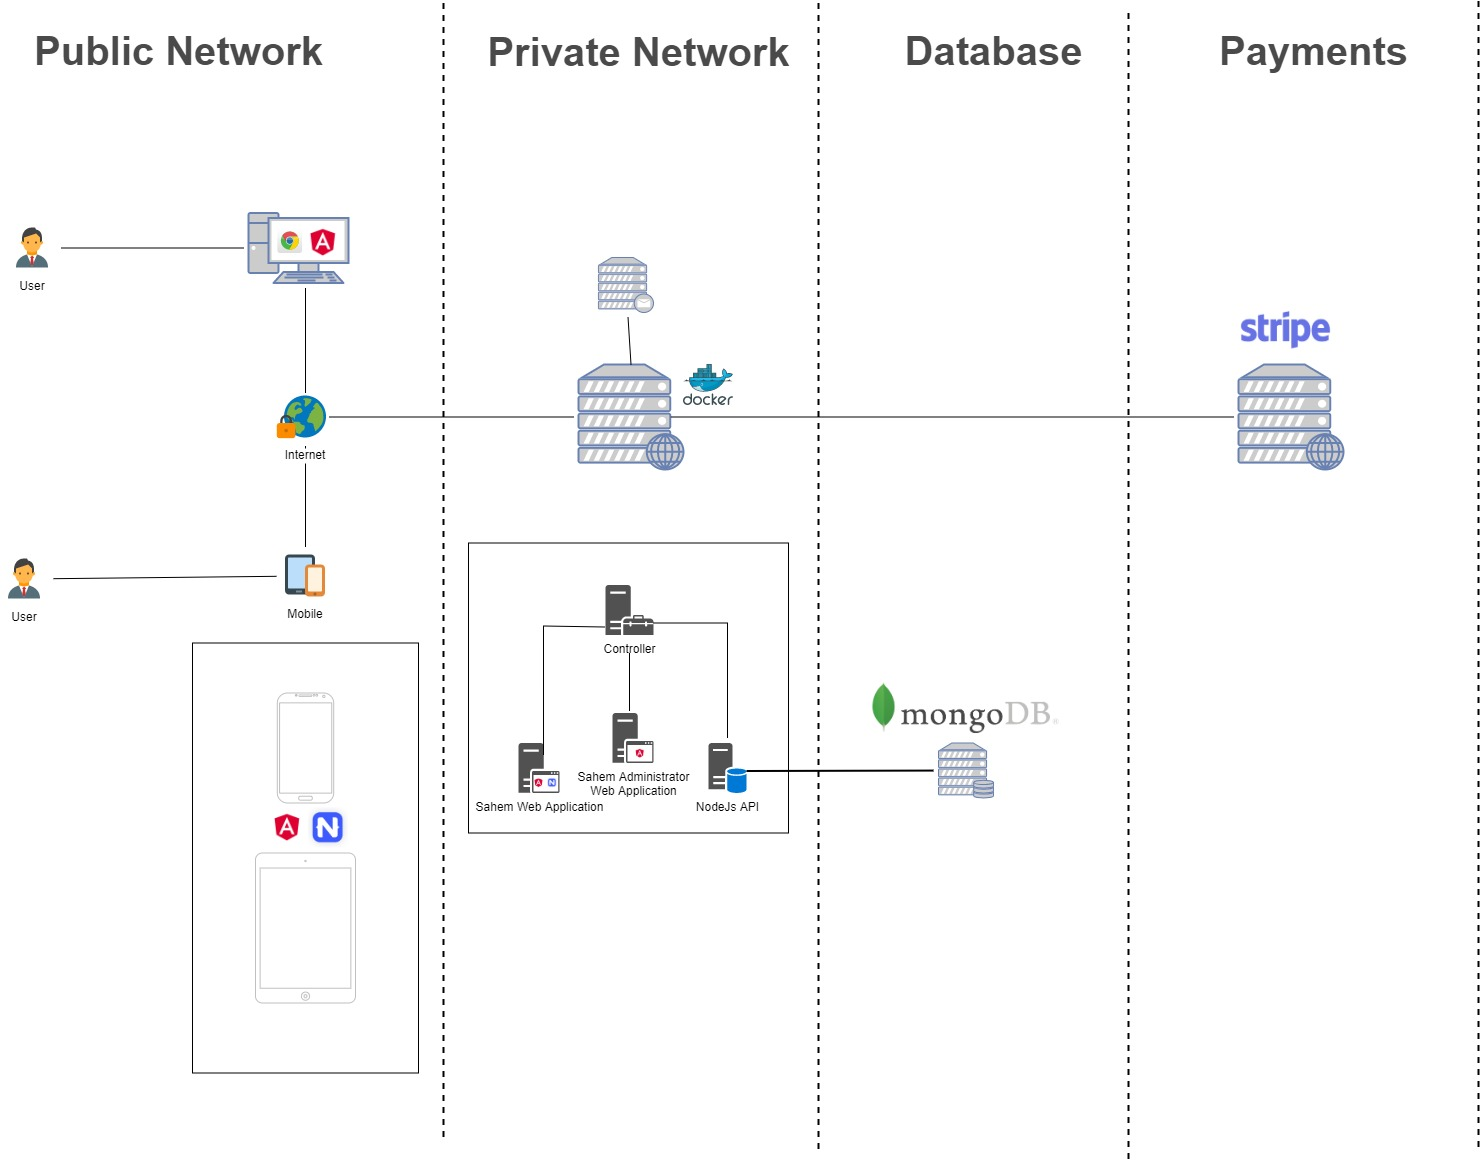
\includegraphics[scale=0.30]{assets/architecturedrawio.jpg}
      \caption{Sahem Platform's Hardware Architecture}
      \label{fig:sahemarchitecturedrawio}
\end{figure}
This model is the commonly go with model, when it comes to using  Platform as a Service \ac{PaaS} provider for hosting.
\section{Development Environments}
\subsection{Design And Planing}

\paragraph*{PlantUml}
In the modeling phase, we found many other solutions and software that helped to create diagrams, but they all are graphic based solutions, you have to drag and drop a lot of objects, dragging arrows from one class to the other, which we found it to be frustrating and tiring with time, so we have decided to go with PlantUML. We are programmers and we should use that fact.\\
PlantUML is an open-source tool allowing users to create UML diagrams from plain text language. The language of PlantUML is an example of a Domain-specific language. It uses Graphviz software to layout its diagrams. It has been used to allow blind students to work with UML. PlantUML also helps blind software engineers to design and read UML diagrams.


\paragraph*{Gantt chart}
A Gantt chart is a horizontal bar chart that visually represents a project plan over time. Modern Gantt charts typically show us the status of—as well as who’s responsible for—each task in the project.\\

In other words, a Gantt chart is a super-simple way to keep us out of a project pinch!\\

A Gantt chart is made up of several different elements:
\begin{enumerate}
      \item
            Tasklist: Runs vertically down the left of the Gantt chart to describe project work and may be organized into groups and subgroups
      \item
            Timeline: Runs horizontally across the top of the Gantt chart and shows months, weeks, days, and years
      \item
            Dateline: A vertical line that highlights the current date on the Gantt chart
      \item
            Bars: Horizontal markers on the right side of the Gantt chart that represent tasks and show progress, duration, and start and end dates
      \item
            Milestones: Yellow diamonds that call out major events, dates, decisions, and deliverables
      \item
            Dependencies: Light gray lines that connect tasks that need to happen in a certain order
      \item
            Progress: Shows how far along work is and may be indicated by \% Complete and/or bar shading
      \item
            Resource assigned: Indicates the person or team responsible for completing a task
\end{enumerate}


\subsection{User Interface And Product Design}
\paragraph*{Adobe Photoshop}
Adobe Photoshop is a software application for image editing and photo retouching for use on Windows or macOS computers. Photoshop offers users the ability to create, enhance, or otherwise edit images, artwork, and illustrations. Changing backgrounds, simulating a real-life painting, or creating an alternative view of the universe are all possible with Adobe Photoshop. It is the most widely used software tool for photo editing, image manipulation, and retouching for numerous image and video file formats. The tools within Photoshop make it possible to edit both individual images as well as large batches of photos.
We used it to prototype and create our platform logo.
\paragraph*{Adobe XD}
Adobe XD is a vector-based user experience design tool for web apps and mobile apps, developed and published by Adobe Inc. It is available for macOS and Windows, although there are versions for iOS and Android to help preview the result of work directly on mobile devices. XD.






\subsection{Development}
\subsubsection{Version Control}
When building software it’s always important to track your changes. This is especially critical when collaborating on projects where multiple people will be updating the same code. Software that can keep track of all
these changes is called Version Control. The Version Control software we used is called Git. Because we built
the platform for a client we decided to get a private repository at Github.com.

\paragraph*{Git}
% Git is a version control system for tracking changes in computer files and coordinating work on those files among multiple people. It is primarily used for source code management in software development, but it can be used to keep track of changes in any set of files. As a distributed revision control system it is aimed at speed, data integrity, and support for distributed, non-linear workflows.
Git is a distributed revision control and source code management system that
allows several people to work on the same codebase at the same time on different
computers and networks. These can be pushed together, with all changes stored and
recorded. It’s also possible to roll back to an earlier state if necessary.
\paragraph*{Github}
At a high level, GitHub is a website and cloud-based service that helps developers store and manage their code, as well as track and control changes to their code. To understand exactly what GitHub is, we need to know two connected principles:
\begin{enumerate}
      \item Version control
      \item Git
\end{enumerate}

\paragraph{Github Desktop}
GitHub Desktop is a fast and easy way to contribute to projects from Windows and OS X, whether we are seasoned users or new users, GitHub Desktop is designed to simplify all processes and workflow in our GitHub. GitHub Desktop is an open-source Electron-based GitHub app. It is written in TypeScript and uses React.


\subsubsection{Dependency Managers}
A large software project often makes use of many third-party packages and libraries. In turn, these packages
often rely on several other packages and so on. To keep track of all these dependencies, software developers
use package managers. Below we introduce the ones we have used.
\paragraph*{Node Package Manager}
Node Package Manager \ac{NPM}, is two things: first and foremost, it is an online repository for the publishing of open-source Node.js projects; second, it is a command-line utility for interacting with the said repository that aids in package installation, version management, and dependency management.
\paragraph*{Angular CLI}
The Angular CLI is a command-line interface tool that we use to initialize, develop, scaffold, and maintain Angular applications. 
\subsubsection{IDEs}

\paragraph*{Visual Studio Code}
Visual Studio Code is a source code editor developed by Microsoft for Windows, Linux, and macOS. It includes support for debugging, embedded Git control and GitHub, syntax highlighting, intelligent code completion, snippets, and code refactoring.


\paragraph*{MongoDB Compass Community}
MongoDB Compass is the defacto GUI tool for MongoDB much like MySQL Workbench is MySQL’s associated tool. It allows us to visually explore our data, run ad hoc queries, interact with our data with full CRUD functionality, as well as view and optimize our queries’ performance.


\paragraph*{Postman}
Postman is an interactive and automatic tool for verifying the APIs of our project. Postman is a Google Chrome app for interacting with HTTP APIs. It presents us with a friendly GUI for constructing requests and reading responses. It works on the backend, and makes sure that each API is working as intended.

In Postman, we create a request, and Postman looks at the response to make sure it has the element we want in it. As it is an automation tool, it drastically improves the testing time and quality of the project. It helps in the early detection of bugs that might sprout at later stages and cause more damage to the system.

Postman is the way to streamline the process of API testing. All APIs that we create and deploy first rigorously go through Postman so that any major or show stopper bugs are identified on time and fewer bugs leak through to later stages.




\subsubsection{Report And Presentation}
\paragraph*{Boost Note}
Boostnote is an Open source note-taking app for programmers.
Boostnote is a niche tool because designed for programmers, but we are passionate for it.
It focuses on writing Markdown notes and code snippets quickly, and get organized in a better way.

\paragraph*{Latex}
\latex{} is a tool used to create professional-looking documents. It is based on the WYSIWYM (what we see is what we mean) idea, meaning we only have to focus on the contents of our document and the computer will take care of the formatting. Instead of spacing out text on a page to control formatting, as with Microsoft Word or LibreOffice Writer, users can enter plain text and let LATEX take care of the rest.
\paragraph*{MiKTex}
MiKTeX provides the tools necessary to prepare documents using the TeX/LaTeX markup language, as well as a simple tex editor: TeXworks.

\paragraph*{Tex Live}
TeX Live is intended to be a straightforward way to get up and running with the TeX document production system. It provides a comprehensive TeX system with binaries for most flavors of Unix, including GNU/Linux, macOS, and also Windows. It includes all the major TeX-related programs, macro packages, and fonts that are free software, including support for many languages around the world. Many operating systems provide it via their distributions.



\paragraph*{Markdown}
Markdown is a lightweight markup language with plain-text-formatting syntax. Its design allows it to be converted to many output formats, but the original tool by the same name only supports HTML. Markdown is often used to format readme files, for writing messages in online discussion forums, and to create rich text using a plain text editor.
\paragraph*{Marp}
Marp is the ecosystem to write our presentation with plain Markdown.


% section
% section
% section
\section{Platform security}
Security is a constant worry when it comes to information technology. Data theft, hacking, malware, and a host of other threats are enough to keep any IT professional up at night. In this article, we’ll look at the basic principles and best practices that IT professionals use to keep their systems safe.
\\
When you create a website or application, it means you are ready to show thousands of people on the internet. Your customer/audience may be legit, but some of them will try to tamper your application. So we need to follow the following golden rules:
\begin{enumerate}
      \item 
      “Never trust your audience when it comes to your application’s security”
      \item 
      Always validate the user input before getting it into the server.
      \item 
      Always encode the user inputs before printing them on to the screen.
\end{enumerate}

\subsection{Security Principles}
The main three overarching principles in information security are:
\begin{enumerate}
      \item 
      Confidentiality: This means that information is only being seen or used by people who are authorized to access it.
      \item 
      Integrity: This means that any changes to the information by an unauthorized user are impossible (or at least detected), and changes by authorized users are tracked.
      \item 
      Availability: This means that the information is accessible when authorized users need it.
\end{enumerate}

\subsection{Physical level}
For the Physical level, we will be hosting and deploying our application to an IaaS cloud service, the main reason to use the cloud services is the ability they provide to our application to be decentralized, and available all time.\\
Physical security on IaaS is managed by one or several processes, which include:
\begin{enumerate}
      \item 
      Area security definition
      \item 
      Controlled access to those areas
      \item 
      Uninterrupted power supplies
      \item 
      Monitoring critical parameters
      \item 
      Alarms
      \item 
      Air and particle filtering
      \item 
      Fire protection
      \item 
      Others, such as proper risk and issue management
\end{enumerate}
\subsection{Logical level}
Logical Security consists of software safeguards for an organization's systems, including user identification and password access, authenticating, access rights, and authority levels. These measures are to ensure that only authorized users are able to perform actions or access information in a network or a workstation.
We have implemented multiple levels and layers of security to control the integrity of the data exchanged between our users and Sahem platform, from creating form controls to ensure that the data sent from the user is well structured, and when received on the controller, we created multiple layers and implemented some great middlewares and libraries to help us protect the system from different vulnerabilities.\\
And for the Confidentiality, on the Frontend we put guards on our routes, to only give some specific users the accessibility to the functionalities they have the permission to do, and when a request is received on the controller, we check the user's Identity, and check if they are allowed to take the action requested.
\subsubsection{Stripe Payment API}
Stripe was founded in 2010 with the mission of making it easier to accept payments over the internet. At the time, taking credit cards meant working with a legacy processor or a middleman broker who would provide you with access to a processor.
Stripe has been audited by a PCI-certified auditor and is certified to PCI Service Provider Level 1. This is the most stringent level of certification available in the payments industry. \\
They use the best-in-class security tools and practices to maintain a high level of security at Stripe:
\begin{enumerate}
      \item HTTPS and HSTS for secure connections
      \item Encryption of sensitive data and communication
      \item PGP keys to encrypt your communications with Stripe
\end{enumerate}
\subsubsection{Frontend}
Angular has some great protections against common web-application vulnerabilities and attacks to provide it's applications with a good, and secure experience, preventing cross-site scripting \ac{XSS} that prevent attackers from injecting malicious code into web pages. Such code can then, for example, steal user data (in particular, login data) or perform actions to impersonate the user. This is one of the most common attacks on the web.\\
And has built-in support to help prevent two common HTTP vulnerabilities, cross-site request forgery (\ac{CSRF} or XSRF) and cross-site script inclusion \ac{XSSI}. Both of these must be mitigated primarily on the server-side, but Angular provides helpers to make integration on the client-side easier.

\paragraph*{Route Guards}
Angular’s route guards are interfaces that can tell the router whether or not it should allow navigation to a requested route. They make this decision by looking for a true or false return value from a class that implements the given guard interface.
\paragraph*{Form Control}
This is one of the three fundamental building blocks of Angular. It implements most of the base functionality for accessing the value, validation status, user interactions, and events.
\subsubsection{BackEnd}
Security is really hard to get right on the backend. There are so many different factors to consider, countless different ways to break an application. 
This is just as true with Express applications as it is with any other web framework. There's no instant way to make sure an application won't be taken down by a Denial of Service (DoS) attack because of how it handles one type of user input, or how it routes a specific request.
\paragraph*{Error Handling}
Error handling is considered one of the main factors in creating a good production software for any type of applications, so we have made it our main 
\paragraph*{Check for Vulnerabilities}
There are a few tools in the Node ecosystem that allow easy checking for vulnerabilities in Node and Express application dependencies. These tools are highly valuable in ensuring that no vulnerabilities are currently in the packages an application relies on, and none are added into that application when its packages are updated.
\begin{enumerate}
      \item Snyk
      \item Node Security Project
      \item Retire.js
\end{enumerate}

\paragraph*{Helmet}
\paragraph*{HTTP headers}
The helmet middleware is really like a helmet for our applications. It protects our application by setting up various HTTP headers.
\paragraph*{Session Date}
The express-session middleware stores session data on the server; it only saves the session ID in the cookie itself, not session data.

\paragraph*{cookie-session}
Cookie-session is a simple cookie-based session middleware, that allows storing cookies.It doesn't require any database/resources on the server-side, though the total session data cannot exceed the browser’s max cookie size.

\paragraph*{Authentication}
express-jwt-permissions is a middleware that checks \ac{JWT} tokens for permissions. It is very useful to build a user access control system.

\paragraph*{Data sanitize}
Express-mongo-sanitize is a middleware that sanitizes user-supplied data to prevent MongoDB Operator Injection.

\paragraph*{Errors Logging}
Morgan is a library adds some logging capabilities to our Express API.

\paragraph*{Cross-Origin Resource Sharing}
We will use Cors dependency to configure Express to add headers stating that your API accepts requests coming from other origins. This is known as Cross-Origin Resource Sharing \ac{CORS}.
\paragraph*{Server's Information}
Dotenv is a zero-dependency module that loads environment variables from a .env file into process.env.. Storing configuration in the environment separate from code is based on The Twelve-Factor App methodology \ref{web004}.


% section
% section
% section

\section{Interfaces}
% section
% section
% section

\section{tests}

% Karma for angulars
% Mockgoose for mongoose
% Protractor.js end to end testing

% section
% section
% section
% section

\section{Deployment}


\cleardoublepage%



% % @Author: Taha Bouhsine


%%%%%%%%%%%%%%%%%%%%%%%%%%%%
% CHAPTER                  %
%%%%%%%%%%%%%%%%%%%%%%%%%%%%
\setcounter{mtc}{8}
\chapter{Analysis And Design}%
\label{chap:chapter_two}
\minitoc
%%%%%%%%%%%%%%%%%%%%%%%%%%%%
% SECTION                  %
%%%%%%%%%%%%%%%%%%%%%%%%%%%%
\section{General description of the platform}

% \begin{description}\addtolength{\itemsep}{-0.35\baselineskip}%
%   \item[\textbullet~\bfseries Menu Item] \hfill \\%
%         Menu Description.~\\%
%         {\textbf{Focus topics:~}\emph{Topic one, topic two, topic three, ...}}%
%         %
%   \item[\textbullet~\bfseries Menu Item] \hfill \\%
%         Menu Description.~\\%
%         {\textbf{Focus topics:~}\emph{Topic one, topic two, topic three, ...}}%
%         %
%   \item[\textbullet~\bfseries Menu Item] \hfill \\%
%         Menu Description.~\\%
%         {\textbf{Focus topics:~}\emph{Topic one, topic two, topic three, ...}}%
% \end{description}

% Also bullets such as:%
% \begin{itemize}\addtolength{\itemsep}{-0.35\baselineskip}%
%   \item One%
%   \item Two%
%   \item Three%
%   \item Four%
%   \item \ldots%
% \end{itemize}%
% %

\section{Specification of requirements}
We will proceed according to the UML method which consists of identifying and modeling the various business processes in order to easily migrate to an object architecture from a static and dynamic point of view. This analysis presents a total abstraction being independent of any technology or implementation.

The specification of the needs will allow us to have a better approach of the users, the functionalities, and the relationship between the two. It will be in the form of a use case. For this we will proceed as follows:

Identification of requirements.
Identification of the actors of the system.
Identification of use cases.
Description of use cases.
Grouping of use cases into packages.


\subsection{requirements}
The requirements that we have put on the end-product were divided into basic functionalities and optional functionalities.
The User’s basic functionalities are:
\begin{enumerate}
    \item
          Account management: create an account, login, profile, settings, personal info,
          personal dashboard.
    \item
          Start a campaign: send in a proposal for a campaign (webform).
    \item
          Share function: functionality so that a campaign can be shared within social networks, such as Facebook, Instagram, LinkedIn, Twitter, and potentially Pinterest and Google.
    \item
          Contribution invitation: functionality to send out concrete requests to contribute a certain amount
          within the personal social network.
    \item
          Payment function: contributor should be able to pay their ticket through Credit Card.
    \item
          Review function: contributors should have the opportunity to give reviews about and react to events
          that have taken place.
    \item
          Countdown timer: a timer that shows how much time a campaign has left until it closes.
    \item
          Current overview: each campaign should show for example the number of tickets sold/amount of investors, the amount of money raised so far and the goal amount to be raised.
\end{enumerate}


The User’s optional functionalities are:

\begin{enumerate}
    \item
          Personalized recommendations (recommender system): the system will advise, suggest, or give concrete offers. Logged-in visitors see a personalized recommendation based on social profiles and the
          platform’s web page content and actions.
    \item
          Share option via Whatsapp
    \item
          Online helpdesk: chat possibility with a helpdesk worker.
    \item
          Communication tools: communication possibilities with other members and/or the organization of an
          event via chat.
    \item
          Connection with social media: e.g. Facebook application for special opportunities and/or campaigns
          that enabled even more interaction with the target group.
    \item
          Social login: login with a social account.
    \item
          Wallet: deposit money in your personal wallet, which enables you to make several contributions by
          paying with the money in your wallet.
    \item
          Recruit function: a tool to gather more contributors. A contributor can share a campaign within their
          own personal social networks.
    \item
          Notifications: reminders and/or messages related to upcoming events and updates of events.
    \item
          Mobile App: extra functionalities through the use of a camera and GPS on the actual event: e.g. picture/video upload to the website or live visitor numbers.

    \item
          Agenda/calender: an overview that shows which events will take place on which dates (including events
          that have already taken place).
    \item
          Newsletter: send an overview of the events to members of the platform community or a certain
          selection.
    \item
          Promotion function: functionality to share and promote events on different levels: community (everyone), events (only participants of a specific event), social media (within social networks).
    \item
          Campaign management: management tools for the event organization.
    \item
          Reports/statistics: data analyses, tools for advanced analysis of the web page visits.
\end{enumerate}




\subsection{Identification of actors}
In UML we don't use the term users but actors. A player in a system is an entity external to this system that interacts (data entry, reception of information, etc.) with it. The actors make it possible to define the interface that the system will offer to its environment. And also the actor groups together several users who have the same role. And to find actors it will be necessary to identify the different roles that will have to play its users.
In order to facilitate identification, we can imagine this: everything that is outside and interacts with the system is an actor, everything that is inside is a functionality to be realized.
The different actors of the studied system are \ref{fig:sahemactors}:
\begin{figure}[!ht]
      \centering
      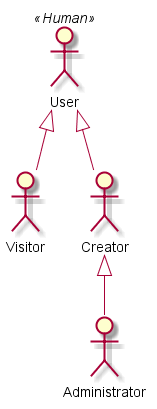
\includegraphics[scale=0.60]{assets/Actors.png}
      \caption{Sahem Platform Actors}
      \label{fig:sahemactors}
\end{figure}
\begin{enumerate}
    \item  Creator.
    \item  Funder will be merged with Creators.
    \item  Administrator.
    \item  Visitor.
\end{enumerate}

\subsection{Identification of objectives and use cases}
A use case described in the form of actions and reactions, the behavior of a system from a user point of view. It must add value to the actor concerned. Each use case contains a list of functionalities that will be detailed in the following section.

We will first determine the objectives that will allow us to deduce the use cases and all this:
\begin{longtable}{|m{10em}|m{10em}|m{10em}|}\hline
    \multirow{4}{*}{Administration management} & \multirow{2}{*}{Authentication}       & Authentication                          \\\cline{3-3}
                                               &                                       & Registration                            \\\cline{2-3}
                                               & \multirow{5}{*}{User Maintainance}    & Add User                                \\\cline{3-3}
                                               &                                       & Modify User                             \\\cline{3-3}
                                               &                                       & Delete User                             \\\cline{3-3}
                                               &                                       & Consult the information of a user       \\\cline{3-3}
                                               &                                       & Show the list of users                  \\\cline{2-3}
                                               & \multirow{2}{*}{Roles}                & Show users by roles                     \\\cline{3-3}
                                               &                                       & Modify a user's role                    \\\cline{2-3}
                                               & \multirow{1}{*}{Statistics}           & Access the statistics of the plateforme \\\hline
    \multirow{4}{*}{Fundraiser's managment}    & \multirow{3}{*}{Creator's Monitoring} & Personal information modification       \\\cline{3-3}
                                               &                                       & Access a creator profile                \\\cline{3-3}
                                               &                                       & Desactivate an Account                  \\\cline{2-3}
                                               & \multirow{2}{*}{Funds Monitoring}     & Fund a project                          \\\cline{3-3}
                                               &                                       & Confirm funding a project               \\\cline{3-3}
                                               &                                       & List of previous funds                  \\\cline{2-3}
                                               & \multirow{6}{*}{Projects Monitoring}  & Create a project                        \\\cline{3-3}
                                               &                                       & Edit a project                          \\\cline{3-3}
                                               &                                       & Delete a project                        \\\cline{3-3}
                                               &                                       & Like a project                          \\\cline{3-3}
                                               &                                       & Share a project                         \\\cline{3-3}
                                               &                                       & Comment on a project                    \\\cline{2-3}
                                               & \multirow{2}{*}{Search}               & Search a project by name                \\\cline{3-3}
                                               &                                       & Show Fundraisers by category            \\\hline
    \multirow{2}{*}{Payment management}        & \multirow{1}{*}{Billing}              & Show the bill                           \\\cline{2-3}
                                               & \multirow{1}{*}{Online Payment}       & Choose payment method                   \\\hline

    \caption{Identification of objectives and use cases}
    \label{tab:id_objec_uc}
\end{longtable}

%%%%%%%%%%%%%%%%%%%%%%%%%%%%
% SECTION                  %
%%%%%%%%%%%%%%%%%%%%%%%%%%%%
\section{Analyse fonctionnelle}
usecase
%%%%%%%%%%%%%%%%%%%%%%%%%%%%
% SECTION                  %
%%%%%%%%%%%%%%%%%%%%%%%%%%%%
\section{Analyse dynamique}
activity  squence
%%%%%%%%%%%%%%%%%%%%%%%%%%%%
% SECTION                  %
%%%%%%%%%%%%%%%%%%%%%%%%%%%%
\section{Analyse structurelle}
class
% \cleardoublepage%

% % @Author: Taha Bouhsine


%%%%%%%%%%%%%%%%%%%%%%%%%%%%
% CHAPTER                  %
%%%%%%%%%%%%%%%%%%%%%%%%%%%%
\setcounter{mtc}{9}

\chapter{Technical and environmental study}%
\label{chap:chapter_tree}
\minitoc
\section{Capture of technical needs}
The capture of technical needs identifies all the constraints and the choices dimensioning the design of the system.

The tools and materials selected as well as the management of integration constraints generally conditioning the prerequisites of general architecture.

The capture of technical needs is as follows:
\begin{itemize}\addtolength{\itemsep}{-0.35\baselineskip}
      \item
            Capturing software specifications.

      \item
            Capturing specifications related to hardware configuration.

\end{itemize}

\subsection{Capturing software specifications}
Once the hardware specifications have been determined, we move on to the non-functional specifications, in other words, technical or software specifications.

These are technical features that the system will provide to the user regardless of the business or functional term.

We will, therefore, list a list of technical functionalities that our system will be able to provide and offer to users, which is why we have introduced the concepts of operator and technical use cases:

\paragraph{Technical actors}
Also called "technical actors" of the system, these are the actors who benefit from the technical functionalities of the system:
\begin{itemize}\addtolength{\itemsep}{-0.35\baselineskip}
      \item
            User: These are the people who use the system functionality in one way or another.
      \item
            Administrator: this is the person responsible for managing all the management of the platform as well as that of the users.
\end{itemize}

\paragraph{Identification of technical use cases}

\begin{longtable}{|m{10em}|m{10em}|m{10em}|}\hline
      \multirow{4}{*}{Security management} & \multirow{5}{*}{Authentication}          & UC1-Register                                                    \\\cline{3-3}
                                           &                                          & UC2-Login                                                       \\\cline{3-3}
                                           &                                          & UC3-Reset Password                                              \\\cline{3-3}
                                           &                                          & UC4-Change password                                             \\\cline{3-3}
                                           &                                          & UC5-Logout                                                      \\\cline{2-3}
                                           & \multirow{1}{*}{Confidentiality}         & UC6-Role management                                             \\\cline{2-3}
                                           & \multirow{2}{*}{Secure payment}          & UC7-Send Payment                                                \\\cline{3-3}
                                           &                                          & UC8-Receive Payment                                             \\\cline{2-3}
                                           & \multirow{2}{*}{Backup and restore}      & UC9-Save the database                                           \\\cline{3-3}
                                           &                                          & UC10-Restore the database                                       \\\hline
      \multirow{7}{*}{Data managment}      & \multirow{1}{*}{Dynamic data}            & UC11-Dynamic data dispaly                                       \\\cline{2-3}
                                           & \multirow{1}{*}{Integrity}               & UC12-Simultaneous updates                                       \\\cline{2-3}
                                           & \multirow{1}{*}{Interoperability}        & UC13-Network deployment                                         \\\cline{2-3}
                                           & \multirow{1}{*}{Compatibility}           & UC14-Run on different browsers and platforms                    \\\cline{2-3}
                                           & \multirow{2}{*}{History}                 & UC15-Get all the user created projects fundraised               \\\cline{3-3}
                                           &                                          & UC16-Get all the user created projects fundraised               \\\cline{2-3}
                                           & \multirow{1}{*}{Statistics}              & UC17-Display platform statistics                                \\\cline{2-3}
                                           & \multirow{1}{*}{Fund}                    & UC18-Fund migration from anonymous user                         \\\hline
      \multirow{4}{*}{Help management}     & \multirow{2}{*}{Gestion des erreurs}     & UC19-Logging Viewing types of errors                            \\\cline{3-3}
                                           &                                          & UC20-Send the error by email to the administrator               \\\cline{2-3}
                                           & \multirow{1}{*}{Aide en ligne}           & UC21-Consult the user help Guide                                \\\cline{2-3}
                                           & \multirow{1}{*}{Notifications}           & UC22-Confirmation or error message                              \\\cline{2-3}
                                           & \multirow{1}{*}{Mails}                   & UC23-Sending emails                                             \\\hline
      \multirow{2}{*}{Payment management}  & \multirow{1}{*}{Multi-currency platform} & UC24-Choose a currency for purchase and payment                 \\\cline{2-3}
                                           & \multirow{1}{*}{Payment method}          & UC25-Possibility to choose a payment method                     \\\hline
      \multirow{3}{*}{Optimization}        & \multirow{1}{*}{Navigation}              & UC26-Nested operations                                          \\\cline{2-3}
                                           & \multirow{1}{*}{Sharing}                 & UC27-Possibility to share your donation                         \\\cline{2-3}
                                           & \multirow{1}{*}{Theming}                 & UC28-Possibility to switch themes between dark and light themes \\\hline

      \caption{Identification of technical objectives and use cases}
      \label{tab:id_tech_objec_uc}
\end{longtable}

\paragraph{ Technical description use cases }
View all the use cases described in the appendix \ref{sec:ucd}


\subsection{Capturing hardware specifications}

\begin{figure}[!ht]
      \centering
      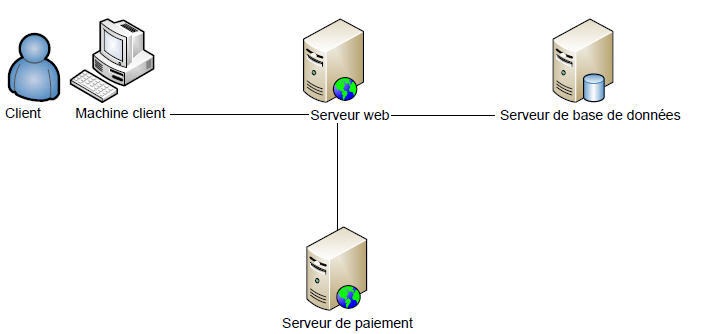
\includegraphics[scale=0.60]{assets/network-arch.jpg}
      \caption{Sahem Platform Actors}
      \label{fig:sahemactors}
\end{figure}

\section{Adopted Architecture}

\subsection{Model View Controller Design Pattern}

The Model View Controller (MVC) design pattern specifies that an application consists of a data model, presentation information, and control information. The pattern requires that each of these be separated into different objects.

MVC is more of an architectural pattern, but not for a complete application. MVC mostly relates to the UI / interaction layer of an application. We’re still going to need a business logic layer, maybe some service layer and data access layer.
\begin{enumerate}
      \item Model contains only the pure application data, it contains no logic describing how to present the data to a user.
      \item View presents the model’s data to the user. The view knows how to access the model’s data, but it does not know what this data means or what the user can do to manipulate it.
      \item Controller exists between the view and the model. It listens to events triggered by the view (or another external source) and executes the appropriate reaction to these events. In most cases, the reaction is to call a method on the model. Since the view and the model are connected through a notification mechanism, the result of this action is then automatically reflected in the view.
\end{enumerate}

\begin{figure}[!ht]
      \center
      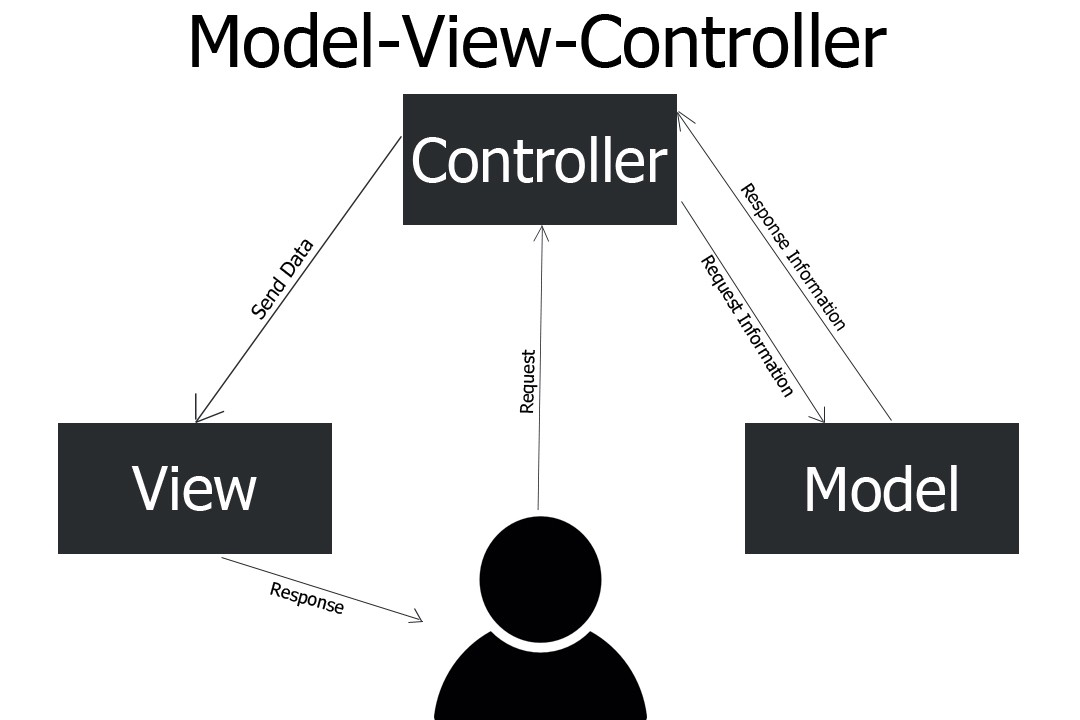
\includegraphics[scale=0.30]{assets/mvc.jpg}
      \caption{Model View Controller}
      \label{fig:mvc}
\end{figure}
% %%%%%%%
\subsection{Representational State Transfer Architecture}
REST, or REpresentational State Transfer, is an architectural style for providing standards between computer systems on the web, making it easier for systems to communicate with each other. REST-compliant systems, often called RESTful systems, are characterized by how they are stateless and separate the concerns of client and server. We will go into what these terms mean and why they are beneficial characteristics for services on the Web.
%%%%
\subsection{Software as a Service}
Software as a Service or SaaS , which allows us to set up services, such as application servers and databases, as needed to create the apps we need. This type of system typically works in a cloud or hybrid cloud environment, which often makes provisioning of servers and software as simple as entering some configurations and clicking a button.

This type of setup is perfect for the MEAN stack, as each piece of the MEAN stack is easily placed into the cloud and thus can be easily provisioned, so they are widely available on SaaS services and can be used quickly when needed. If we are looking for a good development stack, the MEAN stack has much to offer for IT management as well as for developers!
%%%%

\subsection{Monolithic Applications}

If all the functionalities of a project exist in a single codebase, then that application is known as a monolithic application. We all must have designed a monolithic application in our lives in which we were given a problem statement and were asked to design a system with various functionalities. We design our application in various layers like presentation, service, and persistence and then deploy that codebase as a single jar/war file. This is nothing but a monolithic application where “mono” represents the single codebase containing all the required functionalities.
\begin{figure}[!ht]
      \center
      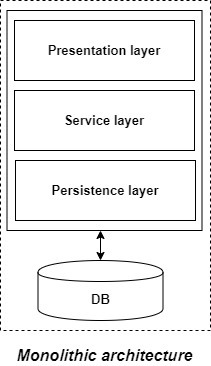
\includegraphics[scale=0.60]{assets/monolithic.jpg}
      \caption{Monolithic Applications}
      \label{fig:monoapp}
\end{figure}

Disadvantages of Monolithic applications:
\begin{enumerate}
      \item
            It becomes too large with time and hence, difficult to manage.
      \item
            We need to redeploy the whole application even for a small change.
      \item
            As the size of the application increases, its start-up and deployment time also increases.
      \item
            For any new developer joining the project, it is very difficult to understand the logic of a large Monolithic application even if his responsibility is related to a single functionality.
      \item
            Even if a single part of the application is facing a large load/traffic, we need to deploy the instances of the whole application in multiple servers. It is very inefficient and takes up more resources unnecessarily. Hence, horizontal scaling is not feasible in monolithic applications.
      \item
            It is very difficult to adopt any new technology which is well suited for a particular functionality as it affects the whole application, both in terms of time and cost.
      \item
            It is not very reliable as a single bug in any module can bring down the whole monolithic application.
\end{enumerate}
Advantages of monolithic applications:
\begin{enumerate}
      \item
            Simple to develop relative to microservices where skilled developers are required in order to identify and develop the services.
      \item
            Easier to deploy as only a single jar/war file is deployed.
      \item
            Relatively easier and simple to develop in comparison to microservices architecture.
      \item
            The problems of network latency and security are relatively less in comparison to microservices architecture.
\end{enumerate}

%%%






% \cleardoublepage%

% Back matter
% @Author: Taha Bouhsine
\setcounter{mtc}{13}

\chapter*{Conclusion}
\label{chap:conclusion}
\minitoc
\markboth{\MakeUppercase{Conclusion}}{}%
\addcontentsline{toc}{chapter}{Conclusion}
 "Ideas are cheap, Execution is expensive" Even if you create a beautiful application with a beautiful User Interface, if you neglect even one aspect of the main functionalities, and built it with a half effort, you might result in a product that won't live for long, or if you were to use the wrong technologies for the project, you might as well find yourself limited and won't be able to create and bring the most out of your Idea.

\cleardoublepage%

% @Author: Taha Bouhsine
\setcounter{mtc}{12}

\chapter*{Appendix}
\label{chap:appendix}
% \minitoc
% \markboth{\MakeUppercase{Appendix}}{}
% \addcontentsline{toc}{chapter}{Appendix}
% \section*{Use cases Description}
% \label{sec:ucd}

% \begin{table}[H]

%   \centering
%   \def\arraystretch{1.5}


%   \begin{tabularx}{\linewidth}{|l|X|X|X|}

%     \hline Use Case \#1                  & \multicolumn{3} {l|}{Register}                                                                          \\ \hline Goal in
%     Description                          & \multicolumn{3}{>{\hsize=\dimexpr 3\hsize+4\tabcolsep+2\arrayrulewidth\relax}X|}{                       %
%       A request from a A2-Visitor to register in the application.  }                                                                               \\
%     \hline Stereotype and Package        &
%     \multicolumn{3}{l|}{« Business » - « User »}                                                                                                   \\
%     \hline Preconditions                 &
%     \multicolumn{3}{l|}{Not registered}                                                                                                            \\
%     \hline Postconditions                &
%     \multicolumn{3}{l|}{Registered}                                                                                                                \\
%     \hline Primary Actors                &
%     \multicolumn{3}{l|}{Visitor}                                                                                                                   \\
%     \hline Use Case Relationships:       &
%     \multicolumn{3}{l|}{Associated with actors A2-Visitor,}                                                                                        \\
%     \hline Basic Flow                    &
%     \multicolumn{3}{l|}{
%       1-The visitor will click on the register button. 2-Fill the personal information form. 2.1- the system will check
%       if the information are valid.
%       3-Fill the payments method form. 3.1- the system will check if the information are valid. 4-Confrm Email.
%       5-System will save the user’s information. 6-System will confrm the users’s registration. 7-redirect the User
%       to the sign in form.}                                                                                                                        \\
%     \hline Alternative Flow              & \multicolumn{3}{l|}{< -information’s are not valid/complete. >}                                         \\


%     \hline Exceptions                    & \multicolumn{3}{l|}{None}                                                                               \\

%     \hline Constraints                   & \multicolumn{3}{l|}{None}                                                                               \\

%     \hline User Interface Specifications & \multicolumn{3}{l|}{}                                                                                   \\

%     \hline \multirow{2}{*}{}             & Metrics                                                                           & Priority & Status   \\
%     \cline{2-4}                          & medium                                                                            & High     & Complete \\
%     \hline Notes                         & \multicolumn{3}{l|}{}                                                                                   \\
%     \hline
%   \end{tabularx}
%   \caption{Use Case Register}
%   \label{tab:use_case_register}
% \end{table}

% \begin{table}[H]

%   \centering
%   \def\arraystretch{1.5}


%   \begin{tabularx}{\linewidth}{|l|X|X|X|}

%     \hline Use Case \#2                  & \multicolumn{3} {l|}{Login}                                                                           \\ \hline Goal in
%     Description                          & \multicolumn{3}{>{\hsize=\dimexpr 3\hsize+4\tabcolsep+2\arrayrulewidth\relax}X|}{                     %
%       A request from a A2-Visitor to the controller to authenticate.  }                                                                          \\
%     \hline Stereotype and Package        &
%     \multicolumn{3}{l|}{« Business » - « Visitor »}                                                                                              \\
%     \hline Preconditions                 &
%     \multicolumn{3}{l|}{Unauthenticated}                                                                                                         \\
%     \hline Postconditions                &
%     \multicolumn{3}{l|}{Authenticated}                                                                                                           \\
%     \hline Primary Actors                &
%     \multicolumn{3}{l|}{Visitor}                                                                                                                 \\
%     \hline Use Case Relationships:       &
%     \multicolumn{3}{l|}{Associated with actors Visitor}                                                                                          \\
%     \hline Basic Flow                    &
%     \multicolumn{3}{l|}{
%       1-The visitor will click on the Login button. 
%       2-Fill the username and password form. 
%         2.1- the system will check if the information are valid. 
%       3-System will log the user’s Session. 
%       4-On success, redirect the User to the main page.}                                                                                                                        \\
%     \hline Alternative Flow              & \multicolumn{3}{l|}{< -information’s are not valid/complete. >}                                                                                 \\


%     \hline Exceptions                    & \multicolumn{3}{l|}{None}                                                                                 \\

%     \hline Constraints                   & \multicolumn{3}{l|}{None}                                                                                 \\

%     \hline User Interface Specifications & \multicolumn{3}{l|}{}                                                                                 \\

%     \hline \multirow{2}{*}{}             & Metrics                                                                           & Priority & Status \\
%     \cline{2-4}                          &  simple                                                                                 & High         & Complete       \\
%     \hline Notes                         & \multicolumn{3}{l|}{}                                                                                 \\
%     \hline
%   \end{tabularx}
%   \caption{Use Case Login}
%   \label{tab:use_case_login}
% \end{table}

% \begin{table}[H]

%   \centering
%   \def\arraystretch{1.5}


%   \begin{tabularx}{\linewidth}{|l|X|X|X|}

%     \hline Use Case \#3                  & \multicolumn{3} {l|}{Reset Password}                                                                  \\ \hline Goal in
%     Description                          & \multicolumn{3}{>{\hsize=\dimexpr 3\hsize+4\tabcolsep+2\arrayrulewidth\relax}X|}{                     %
%     A request from a Visitor to reset the password.  }                                                                                                                    \\
%     \hline Stereotype and Package        &
%     \multicolumn{3}{l|}{« Business » - « Visitor »}                                                                                                                        \\
%     \hline Preconditions                 &
%     \multicolumn{3}{l|}{Old Password}                                                                                                                        \\
%     \hline Postconditions                &
%     \multicolumn{3}{l|}{New Password}                                                                                                                        \\
%     \hline Primary Actors                &
%     \multicolumn{3}{l|}{Visitor}                                                                                                                        \\
%     \hline Use Case Relationships:       &
%     \multicolumn{3}{l|}{Associated with actors Visitor}                                                                                                                        \\
%     \hline Basic Flow                    &
%     \multicolumn{3}{l|}{
%       1-The visitor will click on the Forgot Password button.
%       2-Fill the Email and UserName form. 
%         2.1- the system will check if the information are valid. 
%         2.2- The System will send an reset email to the User Email. 
%     3- the user will click on the link.
%     7- the user will fll the form with the new email. 
%       7.1- check if the password is valid. 
%     8-the user will be redirected to the login page.
%     }                                                                                                                        \\
%     \hline Alternative Flow              & \multicolumn{3}{l|}{ information’s are not valid/complete.}                                                                                 \\


%     \hline Exceptions                    & \multicolumn{3}{l|}{None}                                                                                 \\

%     \hline Constraints                   & \multicolumn{3}{l|}{None}                                                                                 \\

%     \hline User Interface Specifications & \multicolumn{3}{l|}{}                                                                                 \\

%     \hline \multirow{2}{*}{}             & Metrics                                                                           & Priority & Status \\
%     \cline{2-4}                          &  simple                                                                                 &    low      &  Minor      \\
%     \hline Notes                         & \multicolumn{3}{l|}{}                                                                                 \\
%     \hline
%   \end{tabularx}
%   \caption{Use Case Reset Password}
%   \label{tab:use_case_reset_password}
% \end{table}

% \begin{table}[H]

%   \centering
%   \def\arraystretch{1.5}


%   \begin{tabularx}{\linewidth}{|l|X|X|X|}

%     \hline Use Case \#4                  & \multicolumn{3} {l|}{Change password}                                                                 \\ \hline Goal in
%     Description                          & \multicolumn{3}{>{\hsize=\dimexpr 3\hsize+4\tabcolsep+2\arrayrulewidth\relax}X|}{                     %
%       This is a very long line. Lorem ipsum dolor sit amet, consectetur
%       adipiscing elit, sed do eiusmod tempor incididunt ut labore et
%       dolore magna aliqua.  }                                                                                                                    \\
%     \hline Stereotype and Package        &
%     \multicolumn{3}{l|}{}                                                                                                                        \\
%     \hline Preconditions                 &
%     \multicolumn{3}{l|}{}                                                                                                                        \\
%     \hline Postconditions                &
%     \multicolumn{3}{l|}{}                                                                                                                        \\
%     \hline Primary Actors                &
%     \multicolumn{3}{l|}{}                                                                                                                        \\
%     \hline Use Case Relationships:       &
%     \multicolumn{3}{l|}{}                                                                                                                        \\
%     \hline Basic Flow                    &
%     \multicolumn{3}{l|}{}                                                                                                                        \\
%     \hline Alternative Flow              & \multicolumn{3}{l|}{}                                                                                 \\


%     \hline Exceptions                    & \multicolumn{3}{l|}{}                                                                                 \\

%     \hline Constraints                   & \multicolumn{3}{l|}{}                                                                                 \\

%     \hline User Interface Specifications & \multicolumn{3}{l|}{}                                                                                 \\

%     \hline \multirow{2}{*}{}             & Metrics                                                                           & Priority & Status \\
%     \cline{2-4}                          &                                                                                   &          &        \\
%     \hline Notes                         & \multicolumn{3}{l|}{}                                                                                 \\
%     \hline
%   \end{tabularx}
%   \caption{Use Case Change password}
%   \label{tab:use_case_change_password}
% \end{table}

% \begin{table}[H]

%   \centering
%   \def\arraystretch{1.5}


%   \begin{tabularx}{\linewidth}{|l|X|X|X|}

%     \hline Use Case \#5                  & \multicolumn{3} {l|}{Logout}                                                                          \\ \hline Goal in
%     Description                          & \multicolumn{3}{>{\hsize=\dimexpr 3\hsize+4\tabcolsep+2\arrayrulewidth\relax}X|}{                     %
%       This is a very long line. Lorem ipsum dolor sit amet, consectetur
%       adipiscing elit, sed do eiusmod tempor incididunt ut labore et
%       dolore magna aliqua.  }                                                                                                                    \\
%     \hline Stereotype and Package        &
%     \multicolumn{3}{l|}{}                                                                                                                        \\
%     \hline Preconditions                 &
%     \multicolumn{3}{l|}{}                                                                                                                        \\
%     \hline Postconditions                &
%     \multicolumn{3}{l|}{}                                                                                                                        \\
%     \hline Primary Actors                &
%     \multicolumn{3}{l|}{}                                                                                                                        \\
%     \hline Use Case Relationships:       &
%     \multicolumn{3}{l|}{}                                                                                                                        \\
%     \hline Basic Flow                    &
%     \multicolumn{3}{l|}{}                                                                                                                        \\
%     \hline Alternative Flow              & \multicolumn{3}{l|}{}                                                                                 \\


%     \hline Exceptions                    & \multicolumn{3}{l|}{}                                                                                 \\

%     \hline Constraints                   & \multicolumn{3}{l|}{}                                                                                 \\

%     \hline User Interface Specifications & \multicolumn{3}{l|}{}                                                                                 \\

%     \hline \multirow{2}{*}{}             & Metrics                                                                           & Priority & Status \\
%     \cline{2-4}                          &                                                                                   &          &        \\
%     \hline Notes                         & \multicolumn{3}{l|}{}                                                                                 \\
%     \hline
%   \end{tabularx}
%   \caption{Use Case Logout}
%   \label{tab:use_case_logout}
% \end{table}

% \begin{table}[H]

%   \centering
%   \def\arraystretch{1.5}


%   \begin{tabularx}{\linewidth}{|l|X|X|X|}

%     \hline Use Case \#6                  & \multicolumn{3} {l|}{Role management}                                                                 \\ \hline Goal in
%     Description                          & \multicolumn{3}{>{\hsize=\dimexpr 3\hsize+4\tabcolsep+2\arrayrulewidth\relax}X|}{                     %
%       This is a very long line. Lorem ipsum dolor sit amet, consectetur
%       adipiscing elit, sed do eiusmod tempor incididunt ut labore et
%       dolore magna aliqua.  }                                                                                                                    \\
%     \hline Stereotype and Package        &
%     \multicolumn{3}{l|}{}                                                                                                                        \\
%     \hline Preconditions                 &
%     \multicolumn{3}{l|}{}                                                                                                                        \\
%     \hline Postconditions                &
%     \multicolumn{3}{l|}{}                                                                                                                        \\
%     \hline Primary Actors                &
%     \multicolumn{3}{l|}{}                                                                                                                        \\
%     \hline Use Case Relationships:       &
%     \multicolumn{3}{l|}{}                                                                                                                        \\
%     \hline Basic Flow                    &
%     \multicolumn{3}{l|}{}                                                                                                                        \\
%     \hline Alternative Flow              & \multicolumn{3}{l|}{}                                                                                 \\


%     \hline Exceptions                    & \multicolumn{3}{l|}{}                                                                                 \\

%     \hline Constraints                   & \multicolumn{3}{l|}{}                                                                                 \\

%     \hline User Interface Specifications & \multicolumn{3}{l|}{}                                                                                 \\

%     \hline \multirow{2}{*}{}             & Metrics                                                                           & Priority & Status \\
%     \cline{2-4}                          &                                                                                   &          &        \\
%     \hline Notes                         & \multicolumn{3}{l|}{}                                                                                 \\
%     \hline
%   \end{tabularx}
%   \caption{Use Case Role management}
%   \label{tab:use_case_role_management}
% \end{table}

% \begin{table}[H]

%   \centering
%   \def\arraystretch{1.5}


%   \begin{tabularx}{\linewidth}{|l|X|X|X|}

%     \hline Use Case \#7                  & \multicolumn{3} {l|}{Send Payment}                                                                    \\ \hline Goal in
%     Description                          & \multicolumn{3}{>{\hsize=\dimexpr 3\hsize+4\tabcolsep+2\arrayrulewidth\relax}X|}{                     %
%       This is a very long line. Lorem ipsum dolor sit amet, consectetur
%       adipiscing elit, sed do eiusmod tempor incididunt ut labore et
%       dolore magna aliqua.  }                                                                                                                    \\
%     \hline Stereotype and Package        &
%     \multicolumn{3}{l|}{}                                                                                                                        \\
%     \hline Preconditions                 &
%     \multicolumn{3}{l|}{}                                                                                                                        \\
%     \hline Postconditions                &
%     \multicolumn{3}{l|}{}                                                                                                                        \\
%     \hline Primary Actors                &
%     \multicolumn{3}{l|}{}                                                                                                                        \\
%     \hline Use Case Relationships:       &
%     \multicolumn{3}{l|}{}                                                                                                                        \\
%     \hline Basic Flow                    &
%     \multicolumn{3}{l|}{}                                                                                                                        \\
%     \hline Alternative Flow              & \multicolumn{3}{l|}{}                                                                                 \\


%     \hline Exceptions                    & \multicolumn{3}{l|}{}                                                                                 \\

%     \hline Constraints                   & \multicolumn{3}{l|}{}                                                                                 \\

%     \hline User Interface Specifications & \multicolumn{3}{l|}{}                                                                                 \\

%     \hline \multirow{2}{*}{}             & Metrics                                                                           & Priority & Status \\
%     \cline{2-4}                          &                                                                                   &          &        \\
%     \hline Notes                         & \multicolumn{3}{l|}{}                                                                                 \\
%     \hline
%   \end{tabularx}
%   \caption{Use Case Send Payment}
%   \label{tab:use_case_send_payment}
% \end{table}

% \begin{table}[H]

%   \centering
%   \def\arraystretch{1.5}


%   \begin{tabularx}{\linewidth}{|l|X|X|X|}

%     \hline Use Case \#8                  & \multicolumn{3} {l|}{Withdraw Payment}                                                                \\ \hline Goal in
%     Description                          & \multicolumn{3}{>{\hsize=\dimexpr 3\hsize+4\tabcolsep+2\arrayrulewidth\relax}X|}{                     %
%       This is a very long line. Lorem ipsum dolor sit amet, consectetur
%       adipiscing elit, sed do eiusmod tempor incididunt ut labore et
%       dolore magna aliqua.  }                                                                                                                    \\
%     \hline Stereotype and Package        &
%     \multicolumn{3}{l|}{}                                                                                                                        \\
%     \hline Preconditions                 &
%     \multicolumn{3}{l|}{}                                                                                                                        \\
%     \hline Postconditions                &
%     \multicolumn{3}{l|}{}                                                                                                                        \\
%     \hline Primary Actors                &
%     \multicolumn{3}{l|}{}                                                                                                                        \\
%     \hline Use Case Relationships:       &
%     \multicolumn{3}{l|}{}                                                                                                                        \\
%     \hline Basic Flow                    &
%     \multicolumn{3}{l|}{}                                                                                                                        \\
%     \hline Alternative Flow              & \multicolumn{3}{l|}{}                                                                                 \\


%     \hline Exceptions                    & \multicolumn{3}{l|}{}                                                                                 \\

%     \hline Constraints                   & \multicolumn{3}{l|}{}                                                                                 \\

%     \hline User Interface Specifications & \multicolumn{3}{l|}{}                                                                                 \\

%     \hline \multirow{2}{*}{}             & Metrics                                                                           & Priority & Status \\
%     \cline{2-4}                          &                                                                                   &          &        \\
%     \hline Notes                         & \multicolumn{3}{l|}{}                                                                                 \\
%     \hline
%   \end{tabularx}
%   \caption{Use Case withdraw Payment}
%   \label{tab:use_case_withdraw_payment}
% \end{table}

% \begin{table}[H]

%   \centering
%   \def\arraystretch{1.5}


%   \begin{tabularx}{\linewidth}{|l|X|X|X|}

%     \hline Use Case \#9                  & \multicolumn{3} {l|}{Save the database}                                                               \\ \hline Goal in
%     Description                          & \multicolumn{3}{>{\hsize=\dimexpr 3\hsize+4\tabcolsep+2\arrayrulewidth\relax}X|}{                     %
%       This is a very long line. Lorem ipsum dolor sit amet, consectetur
%       adipiscing elit, sed do eiusmod tempor incididunt ut labore et
%       dolore magna aliqua.  }                                                                                                                    \\
%     \hline Stereotype and Package        &
%     \multicolumn{3}{l|}{}                                                                                                                        \\
%     \hline Preconditions                 &
%     \multicolumn{3}{l|}{}                                                                                                                        \\
%     \hline Postconditions                &
%     \multicolumn{3}{l|}{}                                                                                                                        \\
%     \hline Primary Actors                &
%     \multicolumn{3}{l|}{}                                                                                                                        \\
%     \hline Use Case Relationships:       &
%     \multicolumn{3}{l|}{}                                                                                                                        \\
%     \hline Basic Flow                    &
%     \multicolumn{3}{l|}{}                                                                                                                        \\
%     \hline Alternative Flow              & \multicolumn{3}{l|}{}                                                                                 \\


%     \hline Exceptions                    & \multicolumn{3}{l|}{}                                                                                 \\

%     \hline Constraints                   & \multicolumn{3}{l|}{}                                                                                 \\

%     \hline User Interface Specifications & \multicolumn{3}{l|}{}                                                                                 \\

%     \hline \multirow{2}{*}{}             & Metrics                                                                           & Priority & Status \\
%     \cline{2-4}                          &                                                                                   &          &        \\
%     \hline Notes                         & \multicolumn{3}{l|}{}                                                                                 \\
%     \hline
%   \end{tabularx}
%   \caption{Use Case Save the database}
%   \label{tab:use_case_save_the_database}
% \end{table}

% \begin{table}[H]

%   \centering
%   \def\arraystretch{1.5}


%   \begin{tabularx}{\linewidth}{|l|X|X|X|}

%     \hline Use Case \#10                 & \multicolumn{3} {l|}{Restore the database}                                                            \\ \hline Goal in
%     Description                          & \multicolumn{3}{>{\hsize=\dimexpr 3\hsize+4\tabcolsep+2\arrayrulewidth\relax}X|}{                     %
%       This is a very long line. Lorem ipsum dolor sit amet, consectetur
%       adipiscing elit, sed do eiusmod tempor incididunt ut labore et
%       dolore magna aliqua.  }                                                                                                                    \\
%     \hline Stereotype and Package        &
%     \multicolumn{3}{l|}{}                                                                                                                        \\
%     \hline Preconditions                 &
%     \multicolumn{3}{l|}{}                                                                                                                        \\
%     \hline Postconditions                &
%     \multicolumn{3}{l|}{}                                                                                                                        \\
%     \hline Primary Actors                &
%     \multicolumn{3}{l|}{}                                                                                                                        \\
%     \hline Use Case Relationships:       &
%     \multicolumn{3}{l|}{}                                                                                                                        \\
%     \hline Basic Flow                    &
%     \multicolumn{3}{l|}{}                                                                                                                        \\
%     \hline Alternative Flow              & \multicolumn{3}{l|}{}                                                                                 \\


%     \hline Exceptions                    & \multicolumn{3}{l|}{}                                                                                 \\

%     \hline Constraints                   & \multicolumn{3}{l|}{}                                                                                 \\

%     \hline User Interface Specifications & \multicolumn{3}{l|}{}                                                                                 \\

%     \hline \multirow{2}{*}{}             & Metrics                                                                           & Priority & Status \\
%     \cline{2-4}                          &                                                                                   &          &        \\
%     \hline Notes                         & \multicolumn{3}{l|}{}                                                                                 \\
%     \hline
%   \end{tabularx}
%   \caption{Use Case Restore the database}
%   \label{tab:use_case_restore_the_database}
% \end{table}

% \begin{table}[H]

%   \centering
%   \def\arraystretch{1.5}


%   \begin{tabularx}{\linewidth}{|l|X|X|X|}

%     \hline Use Case \#11                 & \multicolumn{3} {l|}{Dynamic data dispaly}                                                            \\ \hline Goal in
%     Description                          & \multicolumn{3}{>{\hsize=\dimexpr 3\hsize+4\tabcolsep+2\arrayrulewidth\relax}X|}{                     %
%       This is a very long line. Lorem ipsum dolor sit amet, consectetur
%       adipiscing elit, sed do eiusmod tempor incididunt ut labore et
%       dolore magna aliqua.  }                                                                                                                    \\
%     \hline Stereotype and Package        &
%     \multicolumn{3}{l|}{}                                                                                                                        \\
%     \hline Preconditions                 &
%     \multicolumn{3}{l|}{}                                                                                                                        \\
%     \hline Postconditions                &
%     \multicolumn{3}{l|}{}                                                                                                                        \\
%     \hline Primary Actors                &
%     \multicolumn{3}{l|}{}                                                                                                                        \\
%     \hline Use Case Relationships:       &
%     \multicolumn{3}{l|}{}                                                                                                                        \\
%     \hline Basic Flow                    &
%     \multicolumn{3}{l|}{}                                                                                                                        \\
%     \hline Alternative Flow              & \multicolumn{3}{l|}{}                                                                                 \\


%     \hline Exceptions                    & \multicolumn{3}{l|}{}                                                                                 \\

%     \hline Constraints                   & \multicolumn{3}{l|}{}                                                                                 \\

%     \hline User Interface Specifications & \multicolumn{3}{l|}{}                                                                                 \\

%     \hline \multirow{2}{*}{}             & Metrics                                                                           & Priority & Status \\
%     \cline{2-4}                          &                                                                                   &          &        \\
%     \hline Notes                         & \multicolumn{3}{l|}{}                                                                                 \\
%     \hline
%   \end{tabularx}
%   \caption{Use Case Dynamic data dispaly}
%   \label{tab:use_case_dynamic_data_dispaly}
% \end{table}

% \begin{table}[H]

%   \centering
%   \def\arraystretch{1.5}


%   \begin{tabularx}{\linewidth}{|l|X|X|X|}

%     \hline Use Case \#12                 & \multicolumn{3} {l|}{Simultaneous updates}                                                            \\ \hline Goal in
%     Description                          & \multicolumn{3}{>{\hsize=\dimexpr 3\hsize+4\tabcolsep+2\arrayrulewidth\relax}X|}{                     %
%       This is a very long line. Lorem ipsum dolor sit amet, consectetur
%       adipiscing elit, sed do eiusmod tempor incididunt ut labore et
%       dolore magna aliqua.  }                                                                                                                    \\
%     \hline Stereotype and Package        &
%     \multicolumn{3}{l|}{}                                                                                                                        \\
%     \hline Preconditions                 &
%     \multicolumn{3}{l|}{}                                                                                                                        \\
%     \hline Postconditions                &
%     \multicolumn{3}{l|}{}                                                                                                                        \\
%     \hline Primary Actors                &
%     \multicolumn{3}{l|}{}                                                                                                                        \\
%     \hline Use Case Relationships:       &
%     \multicolumn{3}{l|}{}                                                                                                                        \\
%     \hline Basic Flow                    &
%     \multicolumn{3}{l|}{}                                                                                                                        \\
%     \hline Alternative Flow              & \multicolumn{3}{l|}{}                                                                                 \\


%     \hline Exceptions                    & \multicolumn{3}{l|}{}                                                                                 \\

%     \hline Constraints                   & \multicolumn{3}{l|}{}                                                                                 \\

%     \hline User Interface Specifications & \multicolumn{3}{l|}{}                                                                                 \\

%     \hline \multirow{2}{*}{}             & Metrics                                                                           & Priority & Status \\
%     \cline{2-4}                          &                                                                                   &          &        \\
%     \hline Notes                         & \multicolumn{3}{l|}{}                                                                                 \\
%     \hline
%   \end{tabularx}
%   \caption{Use Case Simultaneous updates}
%   \label{tab:use_case_simultaneous_updates}
% \end{table}

% \begin{table}[H]

%   \centering
%   \def\arraystretch{1.5}


%   \begin{tabularx}{\linewidth}{|l|X|X|X|}

%     \hline Use Case \#13                 & \multicolumn{3} {l|}{Network deployment}                                                              \\ \hline Goal in
%     Description                          & \multicolumn{3}{>{\hsize=\dimexpr 3\hsize+4\tabcolsep+2\arrayrulewidth\relax}X|}{                     %
%       This is a very long line. Lorem ipsum dolor sit amet, consectetur
%       adipiscing elit, sed do eiusmod tempor incididunt ut labore et
%       dolore magna aliqua.  }                                                                                                                    \\
%     \hline Stereotype and Package        &
%     \multicolumn{3}{l|}{}                                                                                                                        \\
%     \hline Preconditions                 &
%     \multicolumn{3}{l|}{}                                                                                                                        \\
%     \hline Postconditions                &
%     \multicolumn{3}{l|}{}                                                                                                                        \\
%     \hline Primary Actors                &
%     \multicolumn{3}{l|}{}                                                                                                                        \\
%     \hline Use Case Relationships:       &
%     \multicolumn{3}{l|}{}                                                                                                                        \\
%     \hline Basic Flow                    &
%     \multicolumn{3}{l|}{}                                                                                                                        \\
%     \hline Alternative Flow              & \multicolumn{3}{l|}{}                                                                                 \\


%     \hline Exceptions                    & \multicolumn{3}{l|}{}                                                                                 \\

%     \hline Constraints                   & \multicolumn{3}{l|}{}                                                                                 \\

%     \hline User Interface Specifications & \multicolumn{3}{l|}{}                                                                                 \\

%     \hline \multirow{2}{*}{}             & Metrics                                                                           & Priority & Status \\
%     \cline{2-4}                          &                                                                                   &          &        \\
%     \hline Notes                         & \multicolumn{3}{l|}{}                                                                                 \\
%     \hline
%   \end{tabularx}
%   \caption{Use Case Network deployment}
%   \label{tab:use_case_network_deployment}
% \end{table}

% \begin{table}[H]

%   \centering
%   \def\arraystretch{1.5}


%   \begin{tabularx}{\linewidth}{|l|X|X|X|}

%     \hline Use Case \#14                 & \multicolumn{3} {l|}{Run on different browsers and platforms}                                         \\ \hline Goal in
%     Description                          & \multicolumn{3}{>{\hsize=\dimexpr 3\hsize+4\tabcolsep+2\arrayrulewidth\relax}X|}{                     %
%       This is a very long line. Lorem ipsum dolor sit amet, consectetur
%       adipiscing elit, sed do eiusmod tempor incididunt ut labore et
%       dolore magna aliqua.  }                                                                                                                    \\
%     \hline Stereotype and Package        &
%     \multicolumn{3}{l|}{}                                                                                                                        \\
%     \hline Preconditions                 &
%     \multicolumn{3}{l|}{}                                                                                                                        \\
%     \hline Postconditions                &
%     \multicolumn{3}{l|}{}                                                                                                                        \\
%     \hline Primary Actors                &
%     \multicolumn{3}{l|}{}                                                                                                                        \\
%     \hline Use Case Relationships:       &
%     \multicolumn{3}{l|}{}                                                                                                                        \\
%     \hline Basic Flow                    &
%     \multicolumn{3}{l|}{}                                                                                                                        \\
%     \hline Alternative Flow              & \multicolumn{3}{l|}{}                                                                                 \\


%     \hline Exceptions                    & \multicolumn{3}{l|}{}                                                                                 \\

%     \hline Constraints                   & \multicolumn{3}{l|}{}                                                                                 \\

%     \hline User Interface Specifications & \multicolumn{3}{l|}{}                                                                                 \\

%     \hline \multirow{2}{*}{}             & Metrics                                                                           & Priority & Status \\
%     \cline{2-4}                          &                                                                                   &          &        \\
%     \hline Notes                         & \multicolumn{3}{l|}{}                                                                                 \\
%     \hline
%   \end{tabularx}
%   \caption{Use Case Run on different browsers and platforms}
%   \label{tab:use_case_multi_platform}
% \end{table}

% \begin{table}[H]

%   \centering
%   \def\arraystretch{1.5}


%   \begin{tabularx}{\linewidth}{|l|X|X|X|}

%     \hline Use Case \#15                 & \multicolumn{3} {l|}{CRUD Fundraisers}                                                                \\ \hline Goal in
%     Description                          & \multicolumn{3}{>{\hsize=\dimexpr 3\hsize+4\tabcolsep+2\arrayrulewidth\relax}X|}{                     %
%       This is a very long line. Lorem ipsum dolor sit amet, consectetur
%       adipiscing elit, sed do eiusmod tempor incididunt ut labore et
%       dolore magna aliqua.  }                                                                                                                    \\
%     \hline Stereotype and Package        &
%     \multicolumn{3}{l|}{}                                                                                                                        \\
%     \hline Preconditions                 &
%     \multicolumn{3}{l|}{}                                                                                                                        \\
%     \hline Postconditions                &
%     \multicolumn{3}{l|}{}                                                                                                                        \\
%     \hline Primary Actors                &
%     \multicolumn{3}{l|}{}                                                                                                                        \\
%     \hline Use Case Relationships:       &
%     \multicolumn{3}{l|}{}                                                                                                                        \\
%     \hline Basic Flow                    &
%     \multicolumn{3}{l|}{}                                                                                                                        \\
%     \hline Alternative Flow              & \multicolumn{3}{l|}{}                                                                                 \\


%     \hline Exceptions                    & \multicolumn{3}{l|}{}                                                                                 \\

%     \hline Constraints                   & \multicolumn{3}{l|}{}                                                                                 \\

%     \hline User Interface Specifications & \multicolumn{3}{l|}{}                                                                                 \\

%     \hline \multirow{2}{*}{}             & Metrics                                                                           & Priority & Status \\
%     \cline{2-4}                          &                                                                                   &          &        \\
%     \hline Notes                         & \multicolumn{3}{l|}{}                                                                                 \\
%     \hline
%   \end{tabularx}
%   \caption{Use Case CRUD Fundraisers}
%   \label{tab:use_case_fundraisers_crud}
% \end{table}




% \begin{table}[H]

%   \centering
%   \def\arraystretch{1.5}


%   \begin{tabularx}{\linewidth}{|l|X|X|X|}

%     \hline Use Case \#16                 & \multicolumn{3} {l|}{Read the user's funded fundraisers}                                              \\ \hline Goal in
%     Description                          & \multicolumn{3}{>{\hsize=\dimexpr 3\hsize+4\tabcolsep+2\arrayrulewidth\relax}X|}{                     %
%       This is a very long line. Lorem ipsum dolor sit amet, consectetur
%       adipiscing elit, sed do eiusmod tempor incididunt ut labore et
%       dolore magna aliqua.  }                                                                                                                    \\
%     \hline Stereotype and Package        &
%     \multicolumn{3}{l|}{}                                                                                                                        \\
%     \hline Preconditions                 &
%     \multicolumn{3}{l|}{}                                                                                                                        \\
%     \hline Postconditions                &
%     \multicolumn{3}{l|}{}                                                                                                                        \\
%     \hline Primary Actors                &
%     \multicolumn{3}{l|}{}                                                                                                                        \\
%     \hline Use Case Relationships:       &
%     \multicolumn{3}{l|}{}                                                                                                                        \\
%     \hline Basic Flow                    &
%     \multicolumn{3}{l|}{}                                                                                                                        \\
%     \hline Alternative Flow              & \multicolumn{3}{l|}{}                                                                                 \\


%     \hline Exceptions                    & \multicolumn{3}{l|}{}                                                                                 \\

%     \hline Constraints                   & \multicolumn{3}{l|}{}                                                                                 \\

%     \hline User Interface Specifications & \multicolumn{3}{l|}{}                                                                                 \\

%     \hline \multirow{2}{*}{}             & Metrics                                                                           & Priority & Status \\
%     \cline{2-4}                          &                                                                                   &          &        \\
%     \hline Notes                         & \multicolumn{3}{l|}{}                                                                                 \\
%     \hline
%   \end{tabularx}
%   \caption{Use Case Read the user's funded fundraisers}
%   \label{tab:use_case_Read_funded_fundraisers}
% \end{table}

% \begin{table}[H]

%   \centering
%   \def\arraystretch{1.5}


%   \begin{tabularx}{\linewidth}{|l|X|X|X|}

%     \hline Use Case \#17                 & \multicolumn{3} {l|}{Display platform statistics}                                                     \\ \hline Goal in
%     Description                          & \multicolumn{3}{>{\hsize=\dimexpr 3\hsize+4\tabcolsep+2\arrayrulewidth\relax}X|}{                     %
%       This is a very long line. Lorem ipsum dolor sit amet, consectetur
%       adipiscing elit, sed do eiusmod tempor incididunt ut labore et
%       dolore magna aliqua.  }                                                                                                                    \\
%     \hline Stereotype and Package        &
%     \multicolumn{3}{l|}{}                                                                                                                        \\
%     \hline Preconditions                 &
%     \multicolumn{3}{l|}{}                                                                                                                        \\
%     \hline Postconditions                &
%     \multicolumn{3}{l|}{}                                                                                                                        \\
%     \hline Primary Actors                &
%     \multicolumn{3}{l|}{}                                                                                                                        \\
%     \hline Use Case Relationships:       &
%     \multicolumn{3}{l|}{}                                                                                                                        \\
%     \hline Basic Flow                    &
%     \multicolumn{3}{l|}{}                                                                                                                        \\
%     \hline Alternative Flow              & \multicolumn{3}{l|}{}                                                                                 \\


%     \hline Exceptions                    & \multicolumn{3}{l|}{}                                                                                 \\

%     \hline Constraints                   & \multicolumn{3}{l|}{}                                                                                 \\

%     \hline User Interface Specifications & \multicolumn{3}{l|}{}                                                                                 \\

%     \hline \multirow{2}{*}{}             & Metrics                                                                           & Priority & Status \\
%     \cline{2-4}                          &                                                                                   &          &        \\
%     \hline Notes                         & \multicolumn{3}{l|}{}                                                                                 \\
%     \hline
%   \end{tabularx}
%   \caption{Use Case Display platform statistics}
%   \label{tab:use_case_display_platform_statistics}
% \end{table}

% \begin{table}[H]

%   \centering
%   \def\arraystretch{1.5}


%   \begin{tabularx}{\linewidth}{|l|X|X|X|}

%     \hline Use Case \#18                 & \multicolumn{3} {l|}{Fund migration from anonymous user}                                              \\ \hline Goal in
%     Description                          & \multicolumn{3}{>{\hsize=\dimexpr 3\hsize+4\tabcolsep+2\arrayrulewidth\relax}X|}{                     %
%       This is a very long line. Lorem ipsum dolor sit amet, consectetur
%       adipiscing elit, sed do eiusmod tempor incididunt ut labore et
%       dolore magna aliqua.  }                                                                                                                    \\
%     \hline Stereotype and Package        &
%     \multicolumn{3}{l|}{}                                                                                                                        \\
%     \hline Preconditions                 &
%     \multicolumn{3}{l|}{}                                                                                                                        \\
%     \hline Postconditions                &
%     \multicolumn{3}{l|}{}                                                                                                                        \\
%     \hline Primary Actors                &
%     \multicolumn{3}{l|}{}                                                                                                                        \\
%     \hline Use Case Relationships:       &
%     \multicolumn{3}{l|}{}                                                                                                                        \\
%     \hline Basic Flow                    &
%     \multicolumn{3}{l|}{}                                                                                                                        \\
%     \hline Alternative Flow              & \multicolumn{3}{l|}{}                                                                                 \\


%     \hline Exceptions                    & \multicolumn{3}{l|}{}                                                                                 \\

%     \hline Constraints                   & \multicolumn{3}{l|}{}                                                                                 \\

%     \hline User Interface Specifications & \multicolumn{3}{l|}{}                                                                                 \\

%     \hline \multirow{2}{*}{}             & Metrics                                                                           & Priority & Status \\
%     \cline{2-4}                          &                                                                                   &          &        \\
%     \hline Notes                         & \multicolumn{3}{l|}{}                                                                                 \\
%     \hline
%   \end{tabularx}
%   \caption{Use Case Fund migration from anonymous user}
%   \label{tab:use_case_fund_migration_from_anonymous_user}
% \end{table}

% \begin{table}[H]

%   \centering
%   \def\arraystretch{1.5}


%   \begin{tabularx}{\linewidth}{|l|X|X|X|}

%     \hline Use Case \#19                 & \multicolumn{3} {l|}{Logging and Viewing types of errors}                                             \\ \hline Goal in
%     Description                          & \multicolumn{3}{>{\hsize=\dimexpr 3\hsize+4\tabcolsep+2\arrayrulewidth\relax}X|}{                     %
%       This is a very long line. Lorem ipsum dolor sit amet, consectetur
%       adipiscing elit, sed do eiusmod tempor incididunt ut labore et
%       dolore magna aliqua.  }                                                                                                                    \\
%     \hline Stereotype and Package        &
%     \multicolumn{3}{l|}{}                                                                                                                        \\
%     \hline Preconditions                 &
%     \multicolumn{3}{l|}{}                                                                                                                        \\
%     \hline Postconditions                &
%     \multicolumn{3}{l|}{}                                                                                                                        \\
%     \hline Primary Actors                &
%     \multicolumn{3}{l|}{}                                                                                                                        \\
%     \hline Use Case Relationships:       &
%     \multicolumn{3}{l|}{}                                                                                                                        \\
%     \hline Basic Flow                    &
%     \multicolumn{3}{l|}{}                                                                                                                        \\
%     \hline Alternative Flow              & \multicolumn{3}{l|}{}                                                                                 \\


%     \hline Exceptions                    & \multicolumn{3}{l|}{}                                                                                 \\

%     \hline Constraints                   & \multicolumn{3}{l|}{}                                                                                 \\

%     \hline User Interface Specifications & \multicolumn{3}{l|}{}                                                                                 \\

%     \hline \multirow{2}{*}{}             & Metrics                                                                           & Priority & Status \\
%     \cline{2-4}                          &                                                                                   &          &        \\
%     \hline Notes                         & \multicolumn{3}{l|}{}                                                                                 \\
%     \hline
%   \end{tabularx}
%   \caption{Use Case Logging and viewing types of errors}
%   \label{tab:use_case_;ogging_and_viewing_types_of_errors}
% \end{table}

% \begin{table}[H]

%   \centering
%   \def\arraystretch{1.5}


%   \begin{tabularx}{\linewidth}{|l|X|X|X|}

%     \hline Use Case \#20                 & \multicolumn{3} {l|}{Send the error by email to the administrator}                                    \\ \hline Goal in
%     Description                          & \multicolumn{3}{>{\hsize=\dimexpr 3\hsize+4\tabcolsep+2\arrayrulewidth\relax}X|}{                     %
%       This is a very long line. Lorem ipsum dolor sit amet, consectetur
%       adipiscing elit, sed do eiusmod tempor incididunt ut labore et
%       dolore magna aliqua.  }                                                                                                                    \\
%     \hline Stereotype and Package        &
%     \multicolumn{3}{l|}{}                                                                                                                        \\
%     \hline Preconditions                 &
%     \multicolumn{3}{l|}{}                                                                                                                        \\
%     \hline Postconditions                &
%     \multicolumn{3}{l|}{}                                                                                                                        \\
%     \hline Primary Actors                &
%     \multicolumn{3}{l|}{}                                                                                                                        \\
%     \hline Use Case Relationships:       &
%     \multicolumn{3}{l|}{}                                                                                                                        \\
%     \hline Basic Flow                    &
%     \multicolumn{3}{l|}{}                                                                                                                        \\
%     \hline Alternative Flow              & \multicolumn{3}{l|}{}                                                                                 \\


%     \hline Exceptions                    & \multicolumn{3}{l|}{}                                                                                 \\

%     \hline Constraints                   & \multicolumn{3}{l|}{}                                                                                 \\

%     \hline User Interface Specifications & \multicolumn{3}{l|}{}                                                                                 \\

%     \hline \multirow{2}{*}{}             & Metrics                                                                           & Priority & Status \\
%     \cline{2-4}                          &                                                                                   &          &        \\
%     \hline Notes                         & \multicolumn{3}{l|}{}                                                                                 \\
%     \hline
%   \end{tabularx}
%   \caption{Use Case Send the error by email to the administrator}
%   \label{tab:use_case_send_error_by_email_to_the_administrator}
% \end{table}

% \begin{table}[H]

%   \centering
%   \def\arraystretch{1.5}


%   \begin{tabularx}{\linewidth}{|l|X|X|X|}

%     \hline Use Case \#21                 & \multicolumn{3} {l|}{Consult the user help Guide}                                                     \\ \hline Goal in
%     Description                          & \multicolumn{3}{>{\hsize=\dimexpr 3\hsize+4\tabcolsep+2\arrayrulewidth\relax}X|}{                     %
%       This is a very long line. Lorem ipsum dolor sit amet, consectetur
%       adipiscing elit, sed do eiusmod tempor incididunt ut labore et
%       dolore magna aliqua.  }                                                                                                                    \\
%     \hline Stereotype and Package        &
%     \multicolumn{3}{l|}{}                                                                                                                        \\
%     \hline Preconditions                 &
%     \multicolumn{3}{l|}{}                                                                                                                        \\
%     \hline Postconditions                &
%     \multicolumn{3}{l|}{}                                                                                                                        \\
%     \hline Primary Actors                &
%     \multicolumn{3}{l|}{}                                                                                                                        \\
%     \hline Use Case Relationships:       &
%     \multicolumn{3}{l|}{}                                                                                                                        \\
%     \hline Basic Flow                    &
%     \multicolumn{3}{l|}{}                                                                                                                        \\
%     \hline Alternative Flow              & \multicolumn{3}{l|}{}                                                                                 \\


%     \hline Exceptions                    & \multicolumn{3}{l|}{}                                                                                 \\

%     \hline Constraints                   & \multicolumn{3}{l|}{}                                                                                 \\

%     \hline User Interface Specifications & \multicolumn{3}{l|}{}                                                                                 \\

%     \hline \multirow{2}{*}{}             & Metrics                                                                           & Priority & Status \\
%     \cline{2-4}                          &                                                                                   &          &        \\
%     \hline Notes                         & \multicolumn{3}{l|}{}                                                                                 \\
%     \hline
%   \end{tabularx}
%   \caption{Use Case Consult the user help Guide}
%   \label{tab:use_case_consult_the_user_help_Guide}
% \end{table}

% \begin{table}[H]

%   \centering
%   \def\arraystretch{1.5}


%   \begin{tabularx}{\linewidth}{|l|X|X|X|}

%     \hline Use Case \#22                 & \multicolumn{3} {l|}{Confirmation or error message}                                                   \\ \hline Goal in
%     Description                          & \multicolumn{3}{>{\hsize=\dimexpr 3\hsize+4\tabcolsep+2\arrayrulewidth\relax}X|}{                     %
%       This is a very long line. Lorem ipsum dolor sit amet, consectetur
%       adipiscing elit, sed do eiusmod tempor incididunt ut labore et
%       dolore magna aliqua.  }                                                                                                                    \\
%     \hline Stereotype and Package        &
%     \multicolumn{3}{l|}{}                                                                                                                        \\
%     \hline Preconditions                 &
%     \multicolumn{3}{l|}{}                                                                                                                        \\
%     \hline Postconditions                &
%     \multicolumn{3}{l|}{}                                                                                                                        \\
%     \hline Primary Actors                &
%     \multicolumn{3}{l|}{}                                                                                                                        \\
%     \hline Use Case Relationships:       &
%     \multicolumn{3}{l|}{}                                                                                                                        \\
%     \hline Basic Flow                    &
%     \multicolumn{3}{l|}{}                                                                                                                        \\
%     \hline Alternative Flow              & \multicolumn{3}{l|}{}                                                                                 \\


%     \hline Exceptions                    & \multicolumn{3}{l|}{}                                                                                 \\

%     \hline Constraints                   & \multicolumn{3}{l|}{}                                                                                 \\

%     \hline User Interface Specifications & \multicolumn{3}{l|}{}                                                                                 \\

%     \hline \multirow{2}{*}{}             & Metrics                                                                           & Priority & Status \\
%     \cline{2-4}                          &                                                                                   &          &        \\
%     \hline Notes                         & \multicolumn{3}{l|}{}                                                                                 \\
%     \hline
%   \end{tabularx}
%   \caption{Use Case Confirmation or error message}
%   \label{tab:use_case_confirmation_or_error_message}
% \end{table}

% \begin{table}[H]

%   \centering
%   \def\arraystretch{1.5}


%   \begin{tabularx}{\linewidth}{|l|X|X|X|}

%     \hline Use Case \#23                 & \multicolumn{3} {l|}{Sending emails}                                                                  \\ \hline Goal in
%     Description                          & \multicolumn{3}{>{\hsize=\dimexpr 3\hsize+4\tabcolsep+2\arrayrulewidth\relax}X|}{                     %
%       This is a very long line. Lorem ipsum dolor sit amet, consectetur
%       adipiscing elit, sed do eiusmod tempor incididunt ut labore et
%       dolore magna aliqua.  }                                                                                                                    \\
%     \hline Stereotype and Package        &
%     \multicolumn{3}{l|}{}                                                                                                                        \\
%     \hline Preconditions                 &
%     \multicolumn{3}{l|}{}                                                                                                                        \\
%     \hline Postconditions                &
%     \multicolumn{3}{l|}{}                                                                                                                        \\
%     \hline Primary Actors                &
%     \multicolumn{3}{l|}{}                                                                                                                        \\
%     \hline Use Case Relationships:       &
%     \multicolumn{3}{l|}{}                                                                                                                        \\
%     \hline Basic Flow                    &
%     \multicolumn{3}{l|}{}                                                                                                                        \\
%     \hline Alternative Flow              & \multicolumn{3}{l|}{}                                                                                 \\


%     \hline Exceptions                    & \multicolumn{3}{l|}{}                                                                                 \\

%     \hline Constraints                   & \multicolumn{3}{l|}{}                                                                                 \\

%     \hline User Interface Specifications & \multicolumn{3}{l|}{}                                                                                 \\

%     \hline \multirow{2}{*}{}             & Metrics                                                                           & Priority & Status \\
%     \cline{2-4}                          &                                                                                   &          &        \\
%     \hline Notes                         & \multicolumn{3}{l|}{}                                                                                 \\
%     \hline
%   \end{tabularx}
%   \caption{Use Case Sending emails}
%   \label{tab:use_case_sending_emails}
% \end{table}

% \begin{table}[H]

%   \centering
%   \def\arraystretch{1.5}


%   \begin{tabularx}{\linewidth}{|l|X|X|X|}

%     \hline Use Case \#24                 & \multicolumn{3} {l|}{Choose a currency for purchase and payment}                                      \\ \hline Goal in
%     Description                          & \multicolumn{3}{>{\hsize=\dimexpr 3\hsize+4\tabcolsep+2\arrayrulewidth\relax}X|}{                     %
%       This is a very long line. Lorem ipsum dolor sit amet, consectetur
%       adipiscing elit, sed do eiusmod tempor incididunt ut labore et
%       dolore magna aliqua.  }                                                                                                                    \\
%     \hline Stereotype and Package        &
%     \multicolumn{3}{l|}{}                                                                                                                        \\
%     \hline Preconditions                 &
%     \multicolumn{3}{l|}{}                                                                                                                        \\
%     \hline Postconditions                &
%     \multicolumn{3}{l|}{}                                                                                                                        \\
%     \hline Primary Actors                &
%     \multicolumn{3}{l|}{}                                                                                                                        \\
%     \hline Use Case Relationships:       &
%     \multicolumn{3}{l|}{}                                                                                                                        \\
%     \hline Basic Flow                    &
%     \multicolumn{3}{l|}{}                                                                                                                        \\
%     \hline Alternative Flow              & \multicolumn{3}{l|}{}                                                                                 \\


%     \hline Exceptions                    & \multicolumn{3}{l|}{}                                                                                 \\

%     \hline Constraints                   & \multicolumn{3}{l|}{}                                                                                 \\

%     \hline User Interface Specifications & \multicolumn{3}{l|}{}                                                                                 \\

%     \hline \multirow{2}{*}{}             & Metrics                                                                           & Priority & Status \\
%     \cline{2-4}                          &                                                                                   &          &        \\
%     \hline Notes                         & \multicolumn{3}{l|}{}                                                                                 \\
%     \hline
%   \end{tabularx}
%   \caption{Use Case Choose a currency for purchase and payment}
%   \label{tab:use_case_choose_a_currency_for_purchase_and_payment}
% \end{table}

% \begin{table}[H]

%   \centering
%   \def\arraystretch{1.5}


%   \begin{tabularx}{\linewidth}{|l|X|X|X|}

%     \hline Use Case \#25                 & \multicolumn{3} {l|}{Possibility to choose a payment method}                                          \\ \hline Goal in
%     Description                          & \multicolumn{3}{>{\hsize=\dimexpr 3\hsize+4\tabcolsep+2\arrayrulewidth\relax}X|}{                     %
%       This is a very long line. Lorem ipsum dolor sit amet, consectetur
%       adipiscing elit, sed do eiusmod tempor incididunt ut labore et
%       dolore magna aliqua.  }                                                                                                                    \\
%     \hline Stereotype and Package        &
%     \multicolumn{3}{l|}{}                                                                                                                        \\
%     \hline Preconditions                 &
%     \multicolumn{3}{l|}{}                                                                                                                        \\
%     \hline Postconditions                &
%     \multicolumn{3}{l|}{}                                                                                                                        \\
%     \hline Primary Actors                &
%     \multicolumn{3}{l|}{}                                                                                                                        \\
%     \hline Use Case Relationships:       &
%     \multicolumn{3}{l|}{}                                                                                                                        \\
%     \hline Basic Flow                    &
%     \multicolumn{3}{l|}{}                                                                                                                        \\
%     \hline Alternative Flow              & \multicolumn{3}{l|}{}                                                                                 \\


%     \hline Exceptions                    & \multicolumn{3}{l|}{}                                                                                 \\

%     \hline Constraints                   & \multicolumn{3}{l|}{}                                                                                 \\

%     \hline User Interface Specifications & \multicolumn{3}{l|}{}                                                                                 \\

%     \hline \multirow{2}{*}{}             & Metrics                                                                           & Priority & Status \\
%     \cline{2-4}                          &                                                                                   &          &        \\
%     \hline Notes                         & \multicolumn{3}{l|}{}                                                                                 \\
%     \hline
%   \end{tabularx}
%   \caption{Use Case Possibility to choose a payment method}
%   \label{tab:use_case_Possibility to choose a payment method}
% \end{table}

% \begin{table}[H]

%   \centering
%   \def\arraystretch{1.5}


%   \begin{tabularx}{\linewidth}{|l|X|X|X|}

%     \hline Use Case \#26                 & \multicolumn{3} {l|}{Nested operations}                                                               \\ \hline Goal in
%     Description                          & \multicolumn{3}{>{\hsize=\dimexpr 3\hsize+4\tabcolsep+2\arrayrulewidth\relax}X|}{                     %
%       This is a very long line. Lorem ipsum dolor sit amet, consectetur
%       adipiscing elit, sed do eiusmod tempor incididunt ut labore et
%       dolore magna aliqua.  }                                                                                                                    \\
%     \hline Stereotype and Package        &
%     \multicolumn{3}{l|}{}                                                                                                                        \\
%     \hline Preconditions                 &
%     \multicolumn{3}{l|}{}                                                                                                                        \\
%     \hline Postconditions                &
%     \multicolumn{3}{l|}{}                                                                                                                        \\
%     \hline Primary Actors                &
%     \multicolumn{3}{l|}{}                                                                                                                        \\
%     \hline Use Case Relationships:       &
%     \multicolumn{3}{l|}{}                                                                                                                        \\
%     \hline Basic Flow                    &
%     \multicolumn{3}{l|}{}                                                                                                                        \\
%     \hline Alternative Flow              & \multicolumn{3}{l|}{}                                                                                 \\


%     \hline Exceptions                    & \multicolumn{3}{l|}{}                                                                                 \\

%     \hline Constraints                   & \multicolumn{3}{l|}{}                                                                                 \\

%     \hline User Interface Specifications & \multicolumn{3}{l|}{}                                                                                 \\

%     \hline \multirow{2}{*}{}             & Metrics                                                                           & Priority & Status \\
%     \cline{2-4}                          &                                                                                   &          &        \\
%     \hline Notes                         & \multicolumn{3}{l|}{}                                                                                 \\
%     \hline
%   \end{tabularx}
%   \caption{Use Case Nested operations}
%   \label{tab:use_case_nested_operations}
% \end{table}

% \begin{table}[H]

%   \centering
%   \def\arraystretch{1.5}


%   \begin{tabularx}{\linewidth}{|l|X|X|X|}

%     \hline Use Case \#27                 & \multicolumn{3} {l|}{Share to social media}                                                           \\ \hline Goal in
%     Description                          & \multicolumn{3}{>{\hsize=\dimexpr 3\hsize+4\tabcolsep+2\arrayrulewidth\relax}X|}{                     %
%       This is a very long line. Lorem ipsum dolor sit amet, consectetur
%       adipiscing elit, sed do eiusmod tempor incididunt ut labore et
%       dolore magna aliqua.  }                                                                                                                    \\
%     \hline Stereotype and Package        &
%     \multicolumn{3}{l|}{}                                                                                                                        \\
%     \hline Preconditions                 &
%     \multicolumn{3}{l|}{}                                                                                                                        \\
%     \hline Postconditions                &
%     \multicolumn{3}{l|}{}                                                                                                                        \\
%     \hline Primary Actors                &
%     \multicolumn{3}{l|}{}                                                                                                                        \\
%     \hline Use Case Relationships:       &
%     \multicolumn{3}{l|}{}                                                                                                                        \\
%     \hline Basic Flow                    &
%     \multicolumn{3}{l|}{}                                                                                                                        \\
%     \hline Alternative Flow              & \multicolumn{3}{l|}{}                                                                                 \\


%     \hline Exceptions                    & \multicolumn{3}{l|}{}                                                                                 \\

%     \hline Constraints                   & \multicolumn{3}{l|}{}                                                                                 \\

%     \hline User Interface Specifications & \multicolumn{3}{l|}{}                                                                                 \\

%     \hline \multirow{2}{*}{}             & Metrics                                                                           & Priority & Status \\
%     \cline{2-4}                          &                                                                                   &          &        \\
%     \hline Notes                         & \multicolumn{3}{l|}{}                                                                                 \\
%     \hline
%   \end{tabularx}
%   \caption{Use Case Share to social media}
%   \label{tab:use_case_share_to_social_media}
% \end{table}

% \begin{table}[H]

%   \centering
%   \def\arraystretch{1.5}


%   \begin{tabularx}{\linewidth}{|l|X|X|X|}

%     \hline Use Case \#28                 & \multicolumn{3} {l|}{Switch UI themes}                                                                \\ \hline Goal in
%     Description                          & \multicolumn{3}{>{\hsize=\dimexpr 3\hsize+4\tabcolsep+2\arrayrulewidth\relax}X|}{                     %
%       This is a very long line. Lorem ipsum dolor sit amet, consectetur
%       adipiscing elit, sed do eiusmod tempor incididunt ut labore et
%       dolore magna aliqua.  }                                                                                                                    \\
%     \hline Stereotype and Package        &
%     \multicolumn{3}{l|}{}                                                                                                                        \\
%     \hline Preconditions                 &
%     \multicolumn{3}{l|}{}                                                                                                                        \\
%     \hline Postconditions                &
%     \multicolumn{3}{l|}{}                                                                                                                        \\
%     \hline Primary Actors                &
%     \multicolumn{3}{l|}{}                                                                                                                        \\
%     \hline Use Case Relationships:       &
%     \multicolumn{3}{l|}{}                                                                                                                        \\
%     \hline Basic Flow                    &
%     \multicolumn{3}{l|}{}                                                                                                                        \\
%     \hline Alternative Flow              & \multicolumn{3}{l|}{}                                                                                 \\


%     \hline Exceptions                    & \multicolumn{3}{l|}{}                                                                                 \\

%     \hline Constraints                   & \multicolumn{3}{l|}{}                                                                                 \\

%     \hline User Interface Specifications & \multicolumn{3}{l|}{}                                                                                 \\

%     \hline \multirow{2}{*}{}             & Metrics                                                                           & Priority & Status \\
%     \cline{2-4}                          &                                                                                   &          &        \\
%     \hline Notes                         & \multicolumn{3}{l|}{}                                                                                 \\
%     \hline
%   \end{tabularx}
%   \caption{Use Case Switch UI themes}
%   \label{tab:use_case_switch_ui_themes}
% \end{table}

% \section*{Architecture}

\cleardoublepage%

% @Author: Taha Bouhsine

%%%%%%%%%%%%%%%%%%%%%%%%%%%%%%%%%%%%%%%%%%%%%%%%%%%%
% Don't touch this, it is auto generated
%%%%%%%%%%%%%%%%%%%%%%%%%%%%%%%%%%%%%%%%%%%%%%%%%%%%
\nocite{*}

\phantomsection{}
\addcontentsline{toc}{chapter}{Webography}
\printbibliography[title={Webography},type=online]

\phantomsection{}
\addcontentsline{toc}{chapter}{Bibliography}
\printbibliography[title={Bibliography},nottype=online]

\cleardoublepage%

% \includepdf[pages={-}]{008-abstract.pdf}
%\include{008-abstract}
\cleardoublepage%

\addtocontents{toc}{\protect\setcounter{tocdepth}{3}}

\end{pfe-fsa}
\end{document}